%%% MEMOIR CLASS %%%
\documentclass[twoside,12pt,openright,final,english]{memoir}
% Memoir Divisions: \book, \part, \chapter, \section, \subsection
% Fine divisions:   \subsubsection, \paragraph \subparagraph.
%%% END MEMOIR CLASS %%%

\setlength{\parskip}{\baselineskip}%
\setlength{\parindent}{0pt}%

\usepackage{float}

\usepackage{graphicx}
% For full size print graphics
\graphicspath{{./images-original/}}

\makeindex
\makeglossary
\usepackage{color}
\usepackage[usenames,dvipsnames,svgnames,table]{xcolor}

%%% PAGE, STOCK, AND MARGIN SIZE %%%
% Lulu 7.44 x 9.68"   18.90 x 24.58cm
\setstocksize{24.58cm}{18.90cm} % { height }{ width }
\settrimmedsize{\stockheight}{\stockwidth}{*}

%\settypeblocksize{ height }{ width }{ ratio }
\settypeblocksize{19.0cm}{*}{*}

%\setlrmarginsandblock{ spine }{ edge }{ ratio }
% make the spine have more space than outer edge
\setlrmarginsandblock{*}{2.5cm}{1.2}

% \setulmargins{ upper }{ lower }{ ratio }
\setulmargins{2.0cm}{*}{*}

% \setheadfoot{ headheight }{ footskip }
\setheadfoot{12pt}{2cm}

\checkandfixthelayout[fixed]
%%% END PAGE, STOCK, AND MARGIN SIZE %%%

%%% INCLUDED FILES %%%
% select which chapters to render:
\newif\iftitle\titletrue
\newif\ifcopyright\copyrighttrue
\newif\ifintro\introtrue %true
\newif\ifgetting\gettingtrue %true
\newif\iffirst\firsttrue %true
\newif\iftuning\tuningtrue %true
\newif\iforganize\organizetrue %true
\newif\ifadvanced\advancedtrue %true
\newif\iftrouble\troubletrue %true
\newif\ifedge\edgetrue %true
\newif\ifsupport\supporttrue %true
\newif\ifcontact\contacttrue %true
\newif\ifcolophon\colophontrue %true

%% or just render everything:
\newif\ifrendereverything\rendereverythingfalse
\ifrendereverything \titletrue \copyrighttrue \introtrue \gettingtrue \firsttrue \tuningtrue \organizetrue \advancedtrue \troubletrue \edgetrue \supporttrue \contacttrue \colophontrue \fi
%%% END INCLUDED FILES %%%

\setcounter{secnumdepth}{3}
\setcounter{tocdepth}{3}

\usepackage[french]{babel}
\usepackage{ucs}

%%% PDFLATEX %%%
\usepackage{etex}

\usepackage[protrusion,expansion,spacing,kerning,babel,final]{microtype}
\usepackage[utf8x]{inputenc}

%%% PAGE STYLE %%%
\makepagestyle{jebstyle}
\pagestyle{jebstyle}
\makeevenhead{jebstyle}{}{\hspace{2em}\itshape\small\leftmark}{} % KLUDGE
\makeoddhead{jebstyle}{}{\scshape\small\rightmark}{}
\makeevenfoot{jebstyle}{}{\hspace{2em}\thepage}{} % KLUDGE
\makeoddfoot{jebstyle}{}{\thepage}{}
%%% END 

%%% jebinski CHAPTER STYLE %%%
\makechapterstyle{jebinski}{%
% Clear out the chapter name (e.g. capítulo)
  \renewcommand*{\printchaptername}{}
% Clear out the chapter number
  \renewcommand*{\printchapternum}{}
% Set chapter font
  \renewcommand*{\chaptitlefont}{\normalfont\large\scshape}
  \renewcommand*{\printchaptertitle}[1]{%
     \hrule\vskip\onelineskip \centering \chaptitlefont{##1}\par}
  \renewcommand*{\afterchaptertitle}{\vskip\onelineskip \hrule\vskip
     \afterchapskip}
}
%%% END jebinski CHAPTER STYLE %%%

%%% FORMATTING KLUDGES %%%
% fewer overfull lines compared with \fussy and fewer obvious
% large interword spaces than with \sloppy.
\midsloppy
% "fix" for Overfull \hbox
%\emergencystretch=8pt
\setlength{\emergencystretch}{3em}
% \tolerance is a paragraph parameter, probably ignored here
\tolerance=5000 % allow looser spacing 
%\tolerance=95000 % allow waaay looser spacing 
% 10000 almost prevents hyphenation. What's default?
\hyphenpenalty=500 % 500 seems reasonable
%the default \flushbottom
%\sloppypar
\setlength{\topskip}{1.6\topskip}
\checkandfixthelayout
%\sloppybottom
\raggedbottom
%%%%%%%% WIDOWS AND ORPHANS %%%%%%%%%%%
\widowpenalty=10000
\clubpenalty=10000
%%%%%%%% END WIDOWS AND ORPHANS %%%%%%%%%%%
%%% END FORMATTING KLUDGES %%%

%%% FOOTNOTES %%%
% no horizontal rule before footnotes:
\let\oldfootnoterule\footnoterule
\renewcommand*{\footnoterule}{}
% This indents the footnote, or it lines up too far to the
% left on the spanish side. The right page note should really
% move over more to the left
% KLUDGE
\setlength{\footmarkwidth}{3.5em}
%%% END FOOTNOTES %%%

%%% Fancy dings %%%
\usepackage{pifont}

%%% DEBUG %%%
%\showoutput
%\typeoutlayout
%\typeoutstandardlayout
%%% END DEBUG %%%


\usepackage[hidelinks]{hyperref}

%%% END OF PREAMBLE %%%

\begin{document}

%%% BEGIN FRONT MATTER %%%
\frontmatter

% Set page numbers to lowercase roman numerals, and reset the count to 1 (no *)
\pagenumbering{roman}

%%% TITLE PAGE %%%
% We want the title to be on the right hand page.
% If we pad a page, it gives us two with openright
\iftitle
{\include{Title}}
\fi
%%% END TITLE PAGE

%%% COPYRIGHT PAGE %%%
\ifcopyright
{\include{Copyright}}
\fi
%%% END COPYRIGHT PAGE %%%


%%% TABLE OF CONTENTS ToC %%%
\maxtocdepth{section}
% Dots
% space between dots
\renewcommand{\cftchapterdotsep}{15}
% dot symbol (default is period)
\renewcommand{\cftdot}{\textperiodcentered}	% centered period
% Set space between each entry in ToC
\setlength{\cftbeforechapterskip}{5pt}  % 5pt % 3pt
\tableofcontents*
%%% END TABLE OF CONTENTS ToC %%%

%%% LIST OF FIGURES %%%
%\addtodef{\listoffigures}{\clearpage\pagestyle{lof}}{}
% Fit all of List of Figures on one page
\renewcommand*{\lofheadstart}{\vspace{1cm}}
\clearpage
\listoffigures*
%%% END LIST OF FIGURES %%%

%%% CHAPTER STYLE %%%
\chapterstyle{jebinski} % defined in preamble
\def\topblockvspace{0.11}

%%% END FRONTMATTER %%%
%%% BEGIN MAINMATTER %%%
\mainmatter*

% Set page numbering to arabic, but don't reset numbering (*)
\pagenumbering*{arabic}

%%% Introduction %%%
\ifgetting
\chapter{\emph{Introduction}}
\thispagestyle{empty}
\markboth{Introduction}{Manuel Utilisateur de Slic3r}
{%!TEX root = Slic3r-Manual.tex

\section{Pr\'esentation} % (fold)
\label{sec:overview}

Slic3r est un outil qui traduit des mod\`eles 3D en instructions interpr\'et\'ees par une imprimante 3D. Il d\'ecoupe le mod\`ele en couches horizontales et g\'en\`ere les chemins appropri\'es pour les combler.

Slic3r est inclus dans plusieurs logiciels: Pronterface, Repetier-host, ReplicatorG, et peut \^etre utilis\'e comme un programme autonome.

Ce manuel fournira des conseils sur la fa\c{c}on d'installer, configurer et utiliser Slic3r afin de produire d'excellentes impressions.

% section overview (end)


\section{Buts \& Philosophie} % (fold)
\label{sec:goals_philosophy}

Slic3r est un projet original commenc\'e en 2011 par Alessandro Ranellucci (alias Sound), qui a utilis\'e sa connaissance approfondie du langage Perl pour cr\'eer une application rapide et facile \`a utiliser. La lisibilit\'e et la maintenabilit\'e du code font partis les objectifs de conception.

Le programme est constamment en cours d'am\'elioration, Alessandro et les autres contributeurs du projet, apportent r\'eguli\`erement de nouvelles fonctionnalit\'es et les corrections de bogues.

% section goals_philosophy (end)


\section{Faire un don} % (fold)
\label{sec:donating}

Slic3r a commenc\'e comme un travail d'un seul homme, d\'evelopp\'e exclusivement par Alessandro \`a ses heures perdues, en tant que d\'eveloppeur ind\'ependant, ce qui a un co\^ut direct pour lui. En lib\'erant g\'en\'ereusement Slic3r au public en tant que logiciel libre , sous licence GPL, il a permis \`a beaucoup de profiter de son travail.

Il est possible de contribuer par un don. Vous trouverez plus de d\'etails \`a l'adresse: \url{http://slic3r.org/donations}.

% section donating (end)

%!TEX root = Slic3r-Manual.tex
\section{Soutien Slic3r} % (fold)
\label{sec:slic3r_support}

\index{community support}
\index{soutien de la communaut\'e}
\index{Freenode}
\index{IRC}
\index{RepRap}
\index{forums}
\index{website}
\index{site web}
\index{blog}

Une vari\'et\'e de ressources est disponible pour fournir un soutien pour Slic3r.
\subsection{Wiki et FAQ} % (fold)
\label{sub:wiki_and_faq}
Le wiki fournit de la documentation \`a jour, et une section FAQ qui peuvent aider \`a r\'epondre des questions ou des probl\`emes.
\begin{itemize}
    \item \url{https://github.com/alexrj/Slic3r/wiki/Documentation}
    \item \url{https://github.com/alexrj/Slic3r/wiki/FAQ}
\end{itemize}
% subsection wiki_and_faq (end)

\subsection{Blog} % (fold)
\label{sub:blog}
Conseils, astuces et avis sont publi\'es sur le blog Slic3r.
\begin{itemize}
    \item \url{http://slic3r.org/blog}
\end{itemize}
% subsection blog (end)

\subsection{IRC} % (fold)
\label{sub:irc}

Pr\'esentes sur le serveur \texttt{irc.freenode.net}, les salles de chat suivantes sont souvent remplis de gens qui peuvent fournir une aide en temps r\'eel:
\begin{itemize}
\item \texttt{\#reprap}: Communaut\'e tr\`es active du projet RepRap avec de nombreux utilisateurs de Slic3r.
\item \texttt{\#slic3r}: Salon de discussion Slic3r o\`u les d\'eveloppeurs de Slic3r et les utilisateurs peuvent donner de l'aide.
\end{itemize}

% subsection irc (end)

\subsection{Forum RepRap.org} % (fold)
\label{sub:reprap_org_forum}


Un forum d\'edi\'e \`a Slic3r existe dans les forums RepRap.
\begin{itemize}
    \item \url{forums.reprap.org/list.php?263}
\end{itemize}

% subsection reprap_org_forum (end)

\subsection{Suivi des anomalies} % (fold)
\label{sub:issue_tracker}

Si un bogue a \'et\'e d\'ecouvert dans le logiciel alors une question peut \^etre soulev\'ee dans le suivi d'anomalie (issue tracker) du projet.

\begin{itemize}
    \item \url{github.com/alexrj/Slic3r/issues}
\end{itemize}

\textbf{S'il vous pla\^it} prenez le temps de lire les questions d\'ej\`a pos\'ees pour voir si le probl\`eme a d\'ej\`a \'et\'e soumis. V\'erifiez \'egalement que le probl\`eme est un bogue dans l'application, des questions d'aide \`a l'utilisation ne doivent pas \^etre poss\'ees ici.

Si le bogue semble \^etre non d\'eclar\'e alors s'il vous pla\^it veuillez lire le guide de rapport de bogue avant de le soumettre: \url{https://github.com/alexrj/Slic3r/wiki/Quick-guide-to-writing-good-bug-reports}.

% subsection issue_tracker (end)

% section slic3r_support (end)
}
\fi
%%% END Introduction %%%

%%% GETTING SLIC3R %%%
\ifgetting
\chapter{\emph{Obtenir Slic3r}}
\thispagestyle{empty}
\markboth{Obtenir Slic3r}{Manuel Utilisateur de Slic3r}
{%!TEX root = Slic3r-Manual.tex
\index{download}
\index{telechargement}
\index{binaries}
\index{binaires}
\index{Source Code}
\index{Code Source}
\index{GitHub}
\index{license}
\index{licence}

\fbox{
	\parbox{\linewidth}{
		Slic3r est un logiciel libre, sous licence GNU Affero General Public License, version 3.
	}
}	

\section{T\'el\'echargement}

\subsection{Slic3r} % (fold)
\label{sub:slic3r}
Slic3r peut \^etre t\'el\'echarg\'e directement \`a partir de: \url{http://slic3r.org/download}.

Des paquets pr\'e-compil\'es sont disponibles pour Windows, Mac OS X et Linux. Les utilisateurs de Windows et Linux peuvent choisir entre 32 et 64 bit versions pour correspondre \`a leur syst\`eme.
% subsection slic3r (end)

\subsection{Manuel} % (fold)
\label{sub:manual}

La derni\`ere version de ce document en anglais, avec le code source {\LaTeX}, peut \'etre trouv\'ee sur: \url{https://github.com/alexrj/Slic3r-Manual}

La derni\`ere version de ce document en fran\c{c}ais, avec le code source {\LaTeX}, peut \'etre trouv\'ee sur: \url{https://github.com/llegoff/Slic3r-Manual-FR}

% subsection manual (end)

\subsection{Code Source} % (fold)
\label{sub:source}

Le code source est disponible via GitHub: \url{https://github.com/alexrj/Slic3r}. Pour plus de d\'etail sur la compilation depuis le code source, voir §\ref{sec:building_from_source} plus bas.

% subsection source (end)

\section{Installer}

\subsection{Windows}

D\'ecompressez le fichier zip t\'el\'echarg\'e, dans un dossier de votre choix, il n'y a pas de script d'installation. Le dossier r\'esultant contient deux ex\'ecutables:
\begin{itemize}
\item \texttt{slic3r.exe} - d\'emarre la version interface graphique.
\item \texttt{slic3r-console.exe} - peut \^etre utilis\'e \`a partir de la ligne de commande.
\end{itemize}

Le fichier zip peut alors \^etre supprim\'e.

\subsection{Mac OS X}

Double-cliquez sur le fichier dmg t\'el\'echarg\'e, une instance de Finder devrait s'ouvrir avec une ic\^one du programme Slic3r. Acc\'edez au r\'epertoire Applications et faites y glisser l'ic\^one Slic3r.
Le fichier dmg peut alors \^etre supprim\'e.

\subsection{Linux}

Extraire l'archive dans un dossier de votre choix.
soit:
\begin{itemize}
\item Lancer Slic3r directement par l'ex\'ecutable Slic3r, trouv\'e dans le r\'epertoire bin, ou
\item Installez Slic3r en ex\'ecutant le fichier ex\'ecutable do-install, \'egalement trouv\'e dans le dossier bin.
\end{itemize}
Le fichier d'archive peut alors \^etre supprim\'e.



\section{Compiler depuis le code source} % (fold)
\label{sec:building_from_source}

Pour les plus t\'em\'eraires, Slic3r peut \^etre compil\'e \`a partir des derniers fichiers sources trouv\'ees sur GitHub\footnote{\url{https://github.com/alexrj/Slic3r}}.

Les instructions les plus r\'ecentes pour la compilation des fichiers sources et l'ex\'ecution peuvent \^etre trouv\'ees sur le wiki Slic3r.

\begin{itemize}
    \item \textbf{GNU Linux} \hfill \url{https://github.com/alexrj/Slic3r/wiki/Running-Slic3r-from-git-on-GNU-Linux}
    \item \textbf{OS X} \hfill \url{https://github.com/alexrj/Slic3r/wiki/Running-Slic3r-from-git-on-OS-X}
    \item \textbf{Windows} \hfill \url{https://github.com/alexrj/Slic3r/wiki/Running-Slic3r-from-git-on-Windows}

\end{itemize}
}
\fi
%%% END GETTING SLIC3R %%%

%%% FIRST PRINT %%%
\ifgetting
\chapter{\emph{D\'ebuter}}
\thispagestyle{empty}
\markboth{D\'ebuter}{Manuel Utilisateur de Slic3r}
{\include{FirstPrint}}
\fi
%%% END FIRST PRINT %%%

%%% SIMPLE MODE %%%
\ifgetting
\chapter{\emph{Mode Simple}}
\thispagestyle{empty}
\markboth{Mode Simple}{Manuel Utilisateur de Slic3r}
{%!TEX root = Slic3r-Manual.tex
\section{Mode Simple} % (fold)
\label{sec:simple_mode}
\index{simple mode}
\index{mode simple}

Slic3r a deux modes de fonctionnement, Simple et Expert. Ceux-ci peuvent \^etre choisis \`a partir de la fen\^etre \texttt{Preferences} (qui se trouve dans le menu  \texttt{File} (fichier) ).

\begin{figure}[ht]
\centering
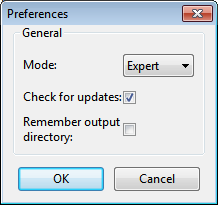
\includegraphics[width=0.3\textwidth]{simple_mode/preferences_general.png}
\caption{Pref\'erences.}
\label{fig:preferences_general}
\end{figure}

Le mode simple offre une gamme r\'eduite de param\`etres, suffisament pour que le d\'ebutant puisse commencer. Le mode expert donne plus de contr\^ole sur la mani\`ere dont Slic3r produit le G-code, celui-ci sera examin\'e plus tard.

\section{Param\`etres d'Impression}
\index{Print Settings}
\index{Param\`etres d'Impression}

L'onglet \texttt{Print Settings} (param\`etres d'impression) 
offre la possibilit\'e de modifier les param\`etres li\'es \`a l'impression r\'eelle. Alors que les autres onglets sont modifi\'ees moins souvent, les param\`etres de cet onglet seront modifi\'es r\'eguli\`erement, \'eventuellement pour chaque mod\`ele imprim\'e.

\begin{figure}[ht]
\centering
\includegraphics[width=\textwidth]{simple_mode/simple_mode_print_settings.png}
\caption{Mode Simple: Param\`etres d'impression.}
\label{fig:simple_mode_print_settings}
\end{figure}

\paragraph{G\'en\'eral.} % (fold)
\label{par:simple_general}
\index{Print Settings!Layer height}
\index{Param\`etres d'Impression!Epaisseur de couche}

\texttt{Layer height} (\'epaisseur de couche) d\'efinit le d\'eplacement sur l'axe vertical avant l'extrusion d'une nouvelle couche.  Il y a plusieurs facteurs qui influentsur la hauteur que la couche doit avoir:
\begin{itemize}
	\item \textbf{R\'esolution D\'esir\'ee}  - Une faible hauteur de couche devrait conduire \`a des impressions avec des nervures ou des bandes moins visibles, comme chaque couche est plus petite. L'esth\'etique joue ici un r\^ole, mais aussi le type de mod\`ele, par exemple, une pi\`ece m\'ecanique peut ne pas avoir besoin d'une telle finition haute r\'esolution, alors qu'une pi\`ece de pr\'esentation peut en avoir besoin.
	\item \textbf{Vitesse d'impression}  - Les couches plus fines produiront des impression lisses, mais chaque impression prendra plus de temps, tout simplement parce que l'extrudeuse doit tracer le motif plusieurs fois. Un des objectifs, plus tard, sera de trouver un \'equilibre entre la hauteur de couche, la vitesse de l'imprimante, et la qualit\'e de l'impression qui en r\'esulte.
\end{itemize}
\index{Print Settings!Perimeters}
\index{Param\`etres d'Impression!P\'erim\`etres}
\texttt{Perimeters} (P\'erim\`etres) d\'efinit le nombre minimum de coquilles verticales (c'est \`a dire les murs) que l'impression aura. \`a moins que le mod\`ele ne n\'ecessite qu'un seul mur, il est g\'en\'eralement recommand\'e d'avoir un minimum de deux p\'erim\`etres car cela donne l'assurance que si une partie du p\'erim\`etre ne s'imprime pas correctement alors le second p\'erim\`etre permettra de le couvrir.

\index{Print Settings!Solid layers}
\index{Param\`etres d'Impression!Couches pleines}
Les couches sup\'erieures et inf\'erieures qui prennent en sandwich le mod\`ele sont remplies de motifs de \texttt{Solid layers} (couches pleines). Pour les couches inf\'erieures (bottom) le facteur important \`a prendre en compte est la façon dont la surface aura l'air s'il y avait une anomalie, lors de l'impression de la premi\`ere couche, c'est pour cette raison, qu'il est recommand\'e d'avoir au moins deux couches inf\'erieures.

Une prise en compte similaire est n\'ecessaire pour les couches sup\'erieures (top). Parce que les couches interm\'ediaires sont susceptibles d'\^etre rempli d'un motif fix\'e \`a moins de 100\% , les couches de rev\^etement devront combler ce motif et cela peut n\'ecessiter plus d'un passage pour le couvrir compl\`etement.

\begin{figure}[H]
\centering
\includegraphics[keepaspectratio=true,width=0.75\textwidth]{simple_mode/bad_top_infill.jpg}
\caption{Un exemple de couches sup\'erieures insuffisantes.}
\label{fig:bad_top_infill}
\end{figure}

Une autre astuce \`a consid\'erer: R\'egler la couche pleine sup\'erieure (top solid layer) \`a z\'ero, et r\'egler le remplissage \'egalement \`a z\'ero, produira un r\'ecipient , id\'eal pour transformer les mod\`eles en vases\footnote{http://slic3r.org/blog/tip-printing-vases} par exemple. Ici la modification des param\`etres peuvent \^etre utilis\'es dans Slic3r pour g\'en\'erer diff\'erents types de impressions, et pas seulement pour contr\^oler la pr\'ecision de surface.

\begin{figure}[H]
\centering
\includegraphics[keepaspectratio=true,width=0.75\textwidth]{simple_mode/solid_layers_vases.png}
\caption{Cr\'eation d'un vase \`a partir d'un mod\`ele solide.}
\label{fig:solid_layers_vases}
\end{figure}

% paragraph general (end)

\paragraph{Remplissage. (Infill)} % (fold)
\label{par:simple_infill}
\index{Print Settings!Infill}
\index{Param\`etres d'Impression!Remplissage}
\index{Print Settings!Infill!Fill density}
\index{Param\`etres d'Impression!Remplissage!Densit\'ee de remplissage}
\texttt{Fill density} (Densit\'e de remplissage) est d\'efinie sur une \'echelle comprise entre 0 et 1, o\`u 1 est de 100\% et 0,4 serait 40\%. Pour la majorit\'e des cas, remplir la pi\`ece \`a 100\% n'a pas d'int\'er\^et, ce serait un gaspillage de mat\'eriel et prendrait beaucoup de temps. Au lieu de cela, la plupart des mod\`eles peuvent \^etre remplis avec moins de mati\`ere, qui sera ensuite pris en sandwich entre les couches remplies \`a 100\% (voir \texttt{Solid layers} au dessus).

Une valeur de densit\'e de 0,4 est suffisant pour donner \`a la quasi-totalit\'e des mod\`eles une bonne r\'esistance m\'ecanique. Une valeur de 0,2 est g\'en\'eralement le minimum requis pour soutenir des plafonds plats.

\index{Print Settings!Infill!Fill pattern}
Slic3r offre plusieurs motifs de remplissage qui seront examin\'es plus en d\'etail dans la section \ref{sec:infill_patterns_and_density} - Motifs et densit\'ee de remplissage.  Choisir un \texttt{Fill pattern} (motif de remplissage) d\'ependra du type de mod\`ele, la r\'esistance souhait\'ee de la structure , la vitesse d'impression, et des go\^uts personnels. Les modes de remplissage plus exotiques sont g\'en\'eralement trop lent et inutilement complexe pour la plupart des cas d'utilisation, et donc la plupart du temps, le motif de remplissage est soit \texttt{rectilinear} (rectiligne), \texttt{line} (ligne), or \texttt{honeycomb} (nid d'abeille).  Honeycomb offre le plus r\'esistance, mais est plus lent que les deux rectilinear ou line.

% paragraph infill (end)

\paragraph{Support. (Support material)} % (fold)
\label{par:simple_support_material}
\index{Print Settings!Support material}
\index{Param\`etres d'Impression!Support}
\index{Print Settings!Support material!Generate support material}
\index{Param\`etres d'Impression!Support!G\'en\'erer le support}
\index{Print Settings!Support material!Pattern spacing}
\index{Param\`etres d'Impression!Support!Espacement du motif}
Imprimer un mod\`ele de bas en haut, avec une imprimante FDM, signifie que les saillies importantes seront imprim\'ees dans le vide, pruduisant des affaissement ou un mauvais r\'esultat.  Obter pour un support (\texttt{Generate support material}) ajoutera des structures suppl\'ementaires dans le mod\`ele qui seront construites pour soutenir la partie en surplomb. Le param\`etre \texttt{Pattern spacing} (espacement du motif) d\'etermine la densit\'e du support qui est imprim\'e.

\begin{figure}[H]
\centering
\includegraphics[keepaspectratio=true,width=0.75\textwidth]{simple_mode/support_example.jpg}
\caption{Un exemple d'un objet imprim\'e avec un support.}
\label{fig:support_example}
\end{figure}

Astuce: Il est parfois utile d'envisager de modifier l'orientation du mod\`ele afin de r\'eduire \'eventuellement les surplombs.

\index{Print Settings!Support material!Raft layers}
\index{Param\`etres d'Impression!Support!Radier}
\texttt{Raft layers} (radier) va ajouter des couches suppl\'ementaires sous le mod\`ele et d\'ecoule depuis les d\'ebuts de l'impression 3D. Il peut vous aider \`a imprimer sans lit chauff\'e, ou lorsque le lit n'est pas tr\`es plat, mais il n'est g\'en\'eralement pas n\'ecessaire et n'est pas recommand\'e. Le radier n\'ecessite en outre un post-traitement pour le supprimer.
% paragraph support_material (end)

\paragraph{Vitesse. (Speed)} % (fold)
\label{par:simple_speed}
\index{Print Settings!Speed}
En mode simple, il n'y a que trois r\'eglages de vitesse \`a configurer:
\index{Print Settings!Speed!Perimeters}
\index{Param\`etres d'Impression!P\'erim\`etres}
\index{Print Settings!Speed!Infill}
\index{Param\`etres d'Impression!Vitesse!Remplissage}
\index{Print Settings!Speed!Travel}
\index{Param\`etres d'Impression!Vitesse!D\'eplacement}
\begin{itemize}
	\item \texttt{Perimeters} (Perimeters) - Le contour du mod\`ele peut b\'en\'eficier d'une vitesse d'impression l\'eg\`erement plus lente de sorte que la peau ext\'erieure de l'impression ait moins de d\'efauts.
	\item \texttt{Remplissage} (Infill) - Comme le remplissage est cach\'e il peut \^etre extrud\'e un peu plus vite. Prenez bien soin de ne pas aller trop vite, car plus la vitesse est \'elev\'ee, et plus les extrusions sont minces, et cela peut affecter la façon dont se fait la liaison entre les extrusions.
	\item \texttt{D\'eplacement} (Travel) - Le saut entre la fin d'une extrusion et la suivante doivent g\'en\'eralement \^etre effectu\'ees aussi rapidement que l'imprimante le permet , afin de minimiser les d\'eg\^ats caus\'es par suintement de mat\'eriau depuis la buse.
\end{itemize}
% paragraph speed (end)

\paragraph{Bordure. (Brim)} % (fold)
\label{par:simple_brim}
\index{Print Settings!Brim}
\index{Param\`etres d'Impression!Bordure}
\index{Print Settings!Brim!Brim width}
\index{Param\`etres d'Impression!Bordure!Largeur de bordure}
\texttt{Brim width} (largeur de bordure) est utilis\'e pour ajouter plus de p\'erim\`etres \`a la premi\`ere couche, en tant base suppl\'ementaire, afin de fournir une plus grande surface pour que l'impression colle au lit , afin de r\'eduire les d\'eformation (voir §\ref{sec:the_important_first_layer}). Le bord est ensuite d\'ecoup\'ee une fois que l'impression est termin\'ee et retir\'ee du lit.

\begin{figure}[H]
\centering
\includegraphics[keepaspectratio=true,width=0.75\textwidth]{simple_mode/brim.jpg}
\caption{Un exemple de bordure.}
\label{fig:an_example_of_brim}
\end{figure}

% paragraph brim (end)

\paragraph{Impression Sequentielle.} % (fold)
\label{par:sequential_printing}
Cette fonction permet de composer un plateau d'objets, en imprimant compl\'etement chaque pi\`ece individuellement, avant de revenir \`a Z = 0 et de continuer par le suivant. Voir la section sur l'impression s\'equentielle dans le chapitre des sujets avanc\'es.


\section{Param\`etres du Filament}
\index{Filament Settings}
\index{Param\`etres du Filament}
L'onglet \texttt{Filament Settings} (Param\`etres du Filament) sera normalement utilis\'e peu fr\'equemment, par exemple lors de la r\'eception d'un nouveau rouleau de filament.

\begin{figure}[H]
\centering
\includegraphics[width=\textwidth]{simple_mode/simple_mode_filament_settings.png}
\caption{Mode Simple: Param\`etres du Filament.}
\label{fig:simple_mode_filament_settings}
\end{figure}

\paragraph{Filament.} % (fold)
\label{par:filament}
\index{Filament Settings!Filament}
\index{Param\`etres du Filament!Filament}
\index{Filament Settings!Filament!Diameter}
\index{Param\`etres du Filament!Filament!Diam\`etre}
Le param\`etre \texttt{Diameter} (Diam\`etre) aura d\'ej\`a \'et\'e rempli \`a partir de la valeur donn\'ee au cours de l'assistant (voir p.\pageref{sub:4_filament_diameter}), mais peut \^etre modifi\'ee ici.

\index{Filament Settings!Filament!Extrusion multiplier}
\index{Param\`etres du Filament!Filament!Multiplicateur d'Extrusion}
La param\`etre \texttt{Extrusion multiplier} (Multiplicateur d'Extrusion) permet le r\'eglage fin de la vitesse d'\'ecoulement d'extrusion, et est est donn\'ee en tant que facteur, par exemple, 1 signifie 100 \%, 1,5 signifierait 150 \%. Alors que la valeur devrait id\'ealement \^etre d\'efinie dans le firmware, il peut \^etre utile de tester l\'eg\`eres modifications de la vitesse en modifiant cette valeur. Elle modifie la quantit\'e de plastique en proportion et doit \^etre chang\'e par de tr\`es petites \'etapes (par exemple + / - 0,05) car les effets sont tr\`es visibles.
% paragraph filament (end)

\paragraph{Temp\'erature.} % (fold)
\label{par:temperature}
\index{Filament Settings!Temperature!Extruder}
\index{Param\`etres du Filament!Temp\'erature!Extrudeuse}
\index{Filament Settings!Temperature!Bed}
\index{Param\`etres du Filament!Temp\'erature!Lit}
Ces valeurs sont \'egalement d\'efinies \`a partir de l'assistant, mais ici la possibilit\'e existe de r\'egler la temp\'erature de la premi\`ere couche (voir p.\pageref{sec:the_important_first_layer}).
% paragraph temperature (end)


\section{Param\`etres de l'Imprimante}
\index{Printer Settings}
\index{Param\`etres de l'Imprimante}

Les param\`etres de l'imprimante (\texttt{Printer Settings}) ne seront jamais mis \`a jour, \`a moins que Slic3r ne soit utilis\'e pour de nombreuses imprimantes, par exemple, pour une batterie de l'imprimante 3D.

\begin{figure}[H]
\centering
\includegraphics[width=\textwidth]{simple_mode/simple_mode_printer_settings.png}
\caption{Mode Simple: Param\`etres de l'Imprimante.}
\label{fig:simple_mode_printer_settings}
\end{figure}

\paragraph{Size and coordinates. (Taille et coordonn\'ees)} % (fold)
\label{par:size_and_coordinates}
\index{Printer Settings!Size and coordinates}
\index{Param\`etres de l'Imprimante!Taille et coordonn\'ees}
\index{Printer Settings!Size and coordinates!Bed size}
\index{Param\`etres de l'Imprimante!Taille et coordonn\'ees!Taille d lit}
Le param\`etre \texttt{Bed size} (Taille du lit) est repris \`a partir de l'assistant (voir p.\pageref{sub:2_bed_size}) et est utilis\'e seulement pour la pr\'evisualisation du mod\`ele sur la surface de travail.

\index{Printer Settings!Size and coordinates!Print center}
\index{Param\`etres de l'Imprimante!Taille et coordonn\'ees!Centre de l'impression}
Le param\`etre \texttt{Print center} (centre de l'impression) defini le point autour duquel l'impression sera centr\'e.  La taille du lit (\texttt{Bed size}) r\'egl\'ee \`a 200mmx200mm et le centre d'impression (\texttt{Print center}) r\'egl\'e \`a 100mmx100mm would placera l'impression au milieu.  Si l'on souhaite imprimer \`a partir du centre, afin d'eviter des bris sur le rebors du verre, cette option doit \^etre utilis\'ee.

\index{Printer Settings!Size and coordinates!Z offset}
\index{Param\`etres de l'Imprimante!Taille et coordonn\'ees!D\'ecalage Z}
\texttt{Z offset} (d\'ecalage Z) peut \^etre utilis\'e pour compenser une fin de course Z mal calibr\'e. Si la buse s'arr\^ete un peu trop loin du lit, on peu conpenser le d\'ecalage en ajoutant une valeur n\'egative. La bonne solution est de r\'egler la but\'ee.

La position de fin de course Z optimale est l\`a o\`u la buse touche \`a peine la surface du lit quand elle se trouve au point d'origine. Une feuille de papier fait un bon indicateur pour cette tr\`es petite distance. Il n'est pas recommand\'e d'utiliser ce param\`etre pour essayer d'am\'eliorer l'adh\'erence couche, en "\'ecrasant" la couche inf\'erieure sur le lit, regardez plut\^ot les suggestions de la section \ref{sec:the_important_first_layer}.
% paragraph size_and_coordinates (end)

\paragraph{Firmware. (Micrologiciel)} % (fold)
\label{par:firmware}
\index{Printer Settings!Firmware!G-code flavour}
\index{Param\`etres de l'Imprimante!Micrologiciel!Variante du G-code}
Comme renseign\'e par l'assistant (voir p.\pageref{sub:1_firmware_type}), \texttt{G-code flavour} (variante du G-code) d\'efinit le dialecte de G-code g\'en\'er\'e.
% paragraph firmware (end)


\paragraph{Extruder. (Extrudeuse)} % (fold)
\label{par:extruder}
\index{Printer Settings!Extruder!Nozzle diameter}
\index{Param\`etres de l'Imprimante!Extrudeuse!Diam\`etre de la buse}
\texttt{Nozzle diameter} (diam\`etre dela buze) est renseign\'e par l'assistant (voir p.\pageref{sub:3_nozzle_diameter}).
% paragraph extruder (end)

\paragraph{Retraction. (Retractation)} % (fold)
\label{par:retraction}
\index{Printer Settings!Extruder!Retraction!Length}
\index{Param\`etres de l'Imprimante!Extrudeuse!R\'etractation!Longueur}
\`a moins que le mat\'eriau en cours d'extrusion ait une viscosit\'e tr\`es \'elev\'ee, il peut suinter entre extrusions dues \`a la pesanteur. Cela peut \^etre r\'esolu en r\'etractant activement le filament entre les extrusions.  R\'egler le param\`etre \texttt{Length} (longueur) \`a une valeur positive causera le filament \`a \^etre retir\'e de plusieurs millim\`etres avant le d\'eplacement. Le retrait sera alors compens\'ee par la m\^eme quantit\'e apr\`es le d\'em\'enagement de Voyage, avant de commencer le nouveau chemin d'extrusion.

Une valeur comprise entre 1 et 2 mm est habituellement recommand\'e. Extrudeuses sous gaine peuvent avoir besoin de 4 ou 5 mm en raison de l'hyst\'er\'esis introduit par le tube.
\index{Printer Settings!Extruder!Retraction!Lift Z}
\index{Param\`etres de l'Imprimante!Extrudeuse!R\'etractation!\'el\'evation Z}
R\'egler le param\`etre \texttt{Lift Z} (El\'evation Z) \`a une valeur positive rel\`evera l'extrudeuse sur l'axe Z de ce nombre de millim\`etres durant chaque d\'eplacement. Cela peut \^etre utile pour s'assurer que la buse n'accroche pas la couche pr\'ecedente, mais cette valeur n'est g\'en\'eralement pas n\'ecessaire et ralentit la vitesse d'impression. Une valeur de 0,1 mm est g\'en\'eralement suffisante.
% paragraph retraction (end)

\paragraph{Start, End and Layer Chance G-codes. (G-code de d\'ebut, de fin et de changement de couche)} % (fold)
\label{par:start_end_g_code}
\index{Printer Settings!Custom G-code!Start G-code}
\index{Param\`etres de l'Imprimante!G-code personnalis\'e!G-code de d\'emarrage}
\index{Printer Settings!Custom G-code!End G-code}
\index{Param\`etres de l'Imprimante!G-code personnalis\'e!G-code de fin}
Les commandes G-code personnalis\'ees peuvent \^etre ex\'ecut\'es avant que l'impression d\'emarre et apr\`es la fin de l'impression.

Des variables d'environements peuvent \^etre ins\'er\'es dans les commandes G-code\footnote{https://github.com/alexrj/Slic3r/wiki/FAQ\#what-placeholders-can-i-use-in-custom-g-code}.  Par exemple [next\_extruder] retournerait l'index de la prochaine extrudeuse.

Le wiki RepRap est une bonne ressource pour en apprendre davantage sur la vari\'et\'e de G-codes disponibles: \texttt{http://reprap.org/wiki/G-code}.

Remarque: Assurez-vous de v\'erifier qu'un G-code utilis\'e est valide pour votre micrologiciel.

Les commandes saisies dans la section \texttt{Start G-code} (G-code de d\'emarrage) 
sont ins\'er\'es au d\'ebut du fichier de sortie, directement apr\`es les instructions de commande de temp\'erature de l'extrudeuse et du lit. Notez que si les commandes de contr\^ole de la temp\'erature sont sp\'ecifi\'es (M104 et M190), alors celles-ci remplaceront les temp\'eratures G-codes introduites par les param\`etres \texttt{Filament}.

Les G-codes courant \`a utiliser avant le d\'ebut d'impression sont:
\begin{itemize}
	\item \textbf{G28}  - Placer chaques axes \`a sa position d'origine.
\end{itemize}


Les G-codes courants \`a utiliser apr\'es la fin de l'impression sont:
\begin{itemize}
	\item \textbf{M104 S0}  - R\`egle la temp\'erature de l'extrudeuse \`a z\'ero.
	\item \textbf{M140 S0} - D\'efinit la temp\'erature du lit chauffant \`a z\'ero.
	\item \textbf{G28 X0} - Place l'axe X \`a son origine.
	\item \textbf{M84}  - D\'esactive les moteurs.
\end{itemize}
% paragraph start_end_g_code (end)

% section simple_mode (end)\section{Simple Mode}
}
\fi
%%% END SIMPLE MODE %%%

%%% EXPERT MODE %%%
\ifadvanced
\chapter{\emph{Mode Expert}}
\thispagestyle{empty}
\markboth{Mode Expert}{Manuel Utilisateur de Slic3r}
{%!TEX root = Slic3r-Manual.tex

\input{Speed}

\newpage

%!TEX root = Slic3r-Manual.tex

\section{Motifs et Densit\'e de Remplissage} % (fold)
\label{sec:infill_patterns_and_density}
\index{infill}
\index{remplissage}

Il y a plusieurs consid\'erations lors du choix d'un motif de remplissage: r\'esistance de l'objet, le temps et la mati\`ere, la pr\'ef\'erence personnelle. On peut en d\'eduire qu'un mod\`ele plus complexe, exigera plus de mouvements, et donc prendra plus de temps et de mati\`ere.
\index{Print Settings!Infill!Fill density}
\index{Param\`etres d'Impression!Remplissage!Densit\'e de remplissage}
\index{Print Settings!Infill!Fill pattern}
\index{Param\`etres d'Impression!Remplissage!Motif de remplissage}
\index{Print Settings!Infill!Fill Top/bottom fill pattern}
\index{Param\`etres d'Impression!Remplissage!Motif de remplissage haut/bas}

\begin{figure}[H]
\centering
\includegraphics[keepaspectratio=true,width=1.0\textwidth]{expertmode/infill_pattern_settings.png}
\caption{R\'eglages des motifs de remplissage.}
\label{fig:infill_pattern_settings}
\end{figure}


Slic3r propose plusieurs mod\`eles de remplissage, quatre commun et trois variantes plus exotiques. Les chiffres indiqu\'es entre parenth\`eses sous chaque figure sont une estimation approximative du mat\'eriau utilis\'e et du temps pris pour un simple mod\`ele de 20 mm cube\footnote{Taken from http://gcode.ws}.  Notez que ce n'est qu'\`a titre indicatif, que la complexit\'e du mod\`ele et d'autres facteurs auront une incidence sur le temps et la mati\`ere.

\begin{figure}[H]
\centering
\includegraphics[keepaspectratio=true,width=0.2\textwidth]{expertmode/infill_line.png}
\caption{Motif de remplissage: Ligne (Line, 344.51mm / 5m:20s)}
\label{fig:infill_line}
\end{figure}

\begin{figure}[H]
\centering
\includegraphics[keepaspectratio=true,width=0.2\textwidth]{expertmode/infill_rectilinear.png}
\caption{Motif de remplissage: Rectiligne (Rectilinear, 350.57mm / 5m:23s)}
\label{fig:infill_rectilinear}
\end{figure}

\begin{figure}[H]
\centering
\includegraphics[keepaspectratio=true,width=0.2\textwidth]{expertmode/infill_concentric.png}
\caption{Motif de remplissage: Concentrique (Concentric, 351.80mm / 5m:30s)}
\label{fig:infill_concentric}
\end{figure}

\begin{figure}[H]
\centering
\includegraphics[keepaspectratio=true,width=0.2\textwidth]{expertmode/infill_honeycomb.png}
\caption{Motif de remplissage: Nid d'abeille (Honeycomb, 362.73mm / 5m:39s)}
\label{fig:infill_honeycomb}
\end{figure}

\begin{figure}[H]
\centering
\includegraphics[keepaspectratio=true,width=0.2\textwidth]{expertmode/infill_hilbertcurve.png}
\caption{Motif de remplissage: Courbe de Hilbert (Hilbert Curve, 332.82mm / 5m:28s)}
\label{fig:infill_hilbertcurve}
\end{figure}

\begin{figure}[H]
\centering
\includegraphics[keepaspectratio=true,width=0.2\textwidth]{expertmode/infill_archimedeanchords.png}
\caption{Motif de remplissage: Cordes d'Archim\`ede (Archimedean Chords, 333.66mm / 5m:27s)}
\label{fig:infill_archimedeanchords}
\end{figure}

\begin{figure}[H]
\centering
\includegraphics[keepaspectratio=true,width=0.2\textwidth]{expertmode/infill_octagramspiral.png}
\caption{Motif de remplissage: Spirale Octogramme (Octagram Spiral, 318.63mm / 5m:15s)}
\label{fig:infill_octagramspiral}
\end{figure}


Certains types de mod\`eles sont plus adapt\'es pour un motif particulier, par exemple le type organique par rapport au type m\'ecanique.  La figure \ref{fig:complex_object_infill_comparison} montre comment un remplissage en nid d'abeilles peut mieux convenir \`a cette pi\`ece m\'ecanique parce que chaque liaisons hexagonales avec la couche pr\'ec\'edente, forment une structure verticale solide.

\begin{figure}[H]
\centering
\includegraphics[keepaspectratio=true,width=0.75\textwidth]{expertmode/complex_object_infill_comparison.png}
\caption{Comparaison de motifs de remplissage pour un objet complexe. De gauche \`a droite: nid d'abeille, ligne}
\label{fig:complex_object_infill_comparison}
\end{figure}


La plupart des mod\`eles ne n\'ecessitent qu'un remplissage de faible densit\'e, en fournissant plus de, disons, 50\% produira un mod\`ele tr\`es serr\'es qui utilise plus de mati\`ere que n\'ecessaire. Pour cette raison, une gamme usuelle de r\'eglages est comprise entre 10\% et 30\%, mais les exigences du mod\`ele permettront de d\'eterminer o\`u la densit\'e sera la meilleure.  La figure \ref{fig:infill_pattern_densities} montre comment les motifs changent au fur et \`a mesure que la densit\'e augmente.
\begin{figure}[H]
\centering
\includegraphics[keepaspectratio=true,width=0.7\textwidth]{expertmode/infills.png}
\caption{ Les motifs de remplissages \`a diff\'erentes densit\'es. de gauche \`a droite: 20\%, 40\%, 60\%, 80\%. De haut en bas: Honeycomb, Concentric, Line, Rectilinear, Hilbert Curve, Archimedean Chords, Octagram Spiral}
\label{fig:infill_pattern_densities}
\end{figure}

% section infill_patterns_and_density (end)


\newpage

%!TEX root = Slic3r-Manual.tex

\section{Optimisation du Remplissage} % (fold)
\label{sec:infill_optimization}
\index{infill}
\index{remplissage}

Slic3r contient plusieurs param\`etres de remplissage avanc\'es qui peuvent aider \`a produire de meilleures extrusions.

\begin{figure}[H]
\centering
\includegraphics[keepaspectratio=true,width=1\textwidth]{expertmode/infill_advanced_settings.png}
\caption{Param\`etres avanc\'es de remplissage.}
\label{fig:infill_settings}
\end{figure}
\index{Print Settings!Infill!Infill every n layers}
\index{Param\`etres d'Impression!Remplissage!Remplissage tous les n couches}
\index{Print Settings!Infill!Only infill where needed}
\index{Param\`etres d'Impression!Remplissage!Remplissage uniquement si n\'ecessaire}
\index{Print Settings!Infill!Solid infill every n layers}
\index{Param\`etres d'Impression!Remplissage!Remplissage plein tous les n couches}
\index{Print Settings!Infill!Fill angle}
\index{Param\`etres d'Impression!Remplissage!Angle de remplissage}
\index{Print Settings!Infill!Solid infill threshold area}
\index{Param\`etres d'Impression!Remplissage!Seuil de l'aire de remplissage plein}
\index{Print Settings!Infill!Only retract when crossing perimeters}
\index{Param\`etres d'Impression!Remplissage!Retrait uniquement lors d'un croisement avec un p\'erim\`etre}
\index{Print Settings!Infill!Infill before perimeters}
\index{Param\`etres d'Impression!Remplissage!Remplissage avant les p\'erim\`etres}

\begin{itemize}
    \item \texttt{Infill every \textit{n} layers} (Remplissage tous les n couches) - Produira remplissage vertical \'eparse en sautant d'un certain nombre de couches. Ceci peut \^etre utilis\'e pour acc\'el\'erer le temps d'impression o\`u le remplissage manquant est acceptable.
    \item \texttt{Only infill where needed} (Remplissage uniquement si n\'ecessaire) - Slic3r analysera le mod\`ele et choisir l'endroit o\`u le remplissage est n\'ecessaire pour soutenir les plafonds internes et les surplombs. Utile pour la r\'eduction du temps et de l'utilisation de la mati\`ere.
    \item \texttt{Solid infill every \textit{n} layers} (Remplissage plein tous les n couches) - Force un motif de remplissage solide sur les couches sp\'ecifi\'ees. Z\'ero pour d\'esactiver cette option.
    \item \texttt{Fill angle} (Angle de remplissage) - Par d\'efaut, le motif de remplissage est orient\'e \`a 45 ° afin de fournir la meilleure adh\'erence aux structures des murs. Extrusions d'intercalaires qui courent \`a c\^ot\'e de p\'erim\`etres sont susceptibles de d\'e-stratifi\'e en situation de stress. Certains mod\`eles peuvent n\'ec\'eciter une rotation de l'angle de remplissage afin d'assurer la direction optimale de l'extrusion.
    \item \texttt{Solid infill threshold area} (Seuil de l'aire de remplissage plein) - Les petites surfaces dans le mod\`ele sont g\'en\'eralement mieux lotis \'etant compl\`etement rempli pour fournir l'int\'egrit\'e structurelle. Toutefois cela prendra plus de temps et de mati\`ere, sans que la cette solidit\'e soit n\'ecessaire. R\'eglez cette option s'adapter aux besoins.
    \item \texttt{Only retract when crossing perimeters} (Retrait uniquement lors d'un croisement avec un p\'erim\`etre) - La r\'etractation, pour emp\^echer le suintement, n'est pas n\'ecessaire si l'extrudeuse reste dans les limites du mod\`ele. Des pr\'ecautions doivent \^etre prises si la mati\`ere d'impression suinte trop, ne pas se r\'etracter peut entra\^iner la perte de mati\`ere assez qui affectera la qualit\'e de l'extrusion ult\'erieure. Cependant, la plupart des imprimantes modernes et des mati\`eres souffrent rarement de tels probl\`emes de suintement extr\^emes.
    \item \texttt{Infill before perimeters} (Remplissage avant les p\'erim\`etres) - Inverse l'ordre dans lequel la couche est imprim\'ee. Habituellement, le p\'erim\`etre est fix\'e dans un premier temps, suivi du remplissage, ce qui est g\'en\'eralement pr\'ef\'erable tant le p\'erim\`etre joue le r\^ole d'une paroi contenant le remplissage.
\end{itemize}


% section infill_optimization (end)


\newpage

%!TEX root = Slic3r-Manual.tex

\section{Combatre le Suintement} % (fold)
\label{sec:fighting_ooze}
\index{ooze}
\index{suintement}
\index{retraction}
\index{retractation}


\`a moins que le mat\'eriau en cours d'extrusion ait une viscosit\'e tr\`es \'elev\'ee, il va suinter de la buse entre les deux extrusions. Il y a plusieurs param\`etres dans Slic3r qui peuvent aider \`a y rem\'edier.

Les param\`etres de retractation, de l'onglet \texttt{Printer} (Imprimante) indiquent \`a l'imprimante de retirer le filament entre les mouvements d'extrusion. Cela peut r\'eduire la pression dans la buse, ce qui r\'eduit suintement. Apr\`es un d\'eplacement, la r\'etractation est invers\'e pour pr\'eparer l'extrudeuse pour la prochaine extrusion.

\begin{figure}[H]
\centering
\includegraphics[keepaspectratio=true,width=1.0\textwidth]{expertmode/retraction_settings.png}
\caption{Param\`etres de retractation.}
\label{fig:retraction_settings}
\end{figure}
\index{Printer Settings!Extruder!Retraction!Length}
\index{Param\`etre de l'Imprimante!Extrudeuse!R\'etractation!Longueur}
\index{Printer Settings!Extruder!Retraction!Lift Z}
\index{Param\`etre de l'Imprimante!Extrudeuse!R\'etractation!Lever Z}
\index{Printer Settings!Extruder!Retraction!Speed}
\index{Param\`etre de l'Imprimante!Extrudeuse!R\'etractation!Vitesse}
\index{Printer Settings!Extruder!Retraction!Extra length on restart}
\index{Param\`etre de l'Imprimante!Extrudeuse!R\'etractation!Longueur suppl\'ementaire au red\'emarrage}
\index{Printer Settings!Extruder!Retraction!Minimum travel after retraction}
\index{Param\`etre de l'Imprimante!Extrudeuse!R\'etractation!D\'eplacement minimum apr\`es r\'etractation}
\index{Printer Settings!Extruder!Retraction!Retract on layer change}
\index{Param\`etre de l'Imprimante!Extrudeuse!R\'etractation!R\'etractation au changement de couche}
\index{Printer Settings!Extruder!Retraction!Wipe before retract}
\index{Param\`etre de l'Imprimante!Extrudeuse!R\'etractation!Essuyer avant r\'etractation}

\begin{itemize}
    \item \texttt{Length} (Longueur) - Le nombre de millim\`etres \`a r\'etracter. A noter que la mesure est effectu\'ee \`a partir du filament brut entrant dans l'extrudeuse. Une valeur comprise entre 1 et 2 mm est habituellement recommand\'e. Les extrudeuses d\'eport\'ees peuvent avoir besoin de 4 ou 5 mm en raison de l'hyst\'er\'esis introduit par le tube.
    \item \texttt{Lift Z} (Lever Z) - Soul\`eve l' extrudeuse sur l'axe Z de quelques millim\`etres pendant chaque d\'eplacement. Cela peut \^etre utile pour s'assurer que la buse n'accroche pas un filament d\'ej\`a d\'epos\'e, mais ceci n'est g\'en\'eralement pas n\'ecessaire et ralentit la vitesse d'impression. Une valeur de 0,1 mm est g\'en\'eralement suffisante.
    \item \texttt{Speed} (Vitesse) - La vitesse \`a laquelle le moteur de l'extrudeuse va retirer le filament. La valeur doit \^etre d\'efinie \`a une vitesse que l'extrudeuse peut g\'erer sans sauter des pas, et il est int\'eressant d'exp\'erimenter plusieurs valeurs pour trouver le retrait le plus rapide possible.
    \item \texttt{Extra length on restart} (Longueur suppl\'ementaire au red\'emarrage) -  Ajoute une longueur suppl\'ementaire de fil apr\`es que le retrait soit compens\'e \`a la fin du d\'eplacement. Ce param\`etre est rarement utilis\'e, mais il le doit, si l'impression montrent des signes de manque de mati\`ere apr\`es la fin du d\'eplacement, alors il peut \^etre utile d'ajouter une petite quantit\'e de mati\`ere suppl\'ementaire.
    \item \texttt{Minimum travel after retraction} (D\'eplacement minimum apr\`es r\'etractation) - D\'eclenchement d'une r\'etractation apr\`es des mouvements tr\`es courts est g\'en\'eralement inutile, car la quantit\'e de suintement est g\'en\'eralement n\'egligeable et il ralentit le temps d'impression.  D\'efinis le nombre de millim\`etres minimum que la buse peut parcourir avant d'envisager une r\'etractation.  Si l'imprimante g\'ere bien le suintement cette valeur peut \^etre augment\'ee \`a 5 ou 6 mm.
    \item \texttt{Retract on layer change} (R\'etractation au changement de couche) - Le mouvement le long de l'axe Z, doit \'egalement \^etre consid\'er\'e lorsqu'il s'agit du suintement, sinon des gouttes peuvent se produire. Il est recommand\'e de laisser ce param\`etre coch\'e.
    \item \texttt{Wipe before retract} (Essuyer avant r\'etractation) - D\'eplace la buse tout en r\'etractant de mani\`ere \`a r\'eduire les risques de formation d'une goutte.
\end{itemize}


En outre, il y a plusieurs param\`etres dans l'onglet \texttt{Print Settings} (Param\`ete de l'Imprimante) qui peuvent aider \`a contr\^oler le suintement.

\begin{itemize}
    \index{Print Settings!Infill!Advanced!Only retract when crossing perimeters}
	\index{Param\`etres d'Impression!Remplissage!Advanc\'e!Retrait seulement lors du croisement avec un p\'erim\`etre}
    \item \texttt{Only retract when crossing perimeters} , Retrait seulement lors du croisement avec uns p\'erim\`etre (Infill - Advanced) (Remplissage - Avanc\'e) - Indique \`a Slic3r de ne r\'etracter que si la buse traverse le bord de l'\^ile qui vient d' \^etre extrud\'ee. De l\'eger suintement dans les murs d'une pi\`ece ne sont pas perçus et peuvent g\'en\'eralement \^etre accept\'ee.
    \index{Print Settings!Layers and perimeters!Quality!Avoid crossing perimeters}
    \index{Param\`etres d'Impression!Couches et p\'erim\`etres!Qualit\'e!Evitez de croiser les p\'erim\`etres}
	\item \texttt{Avoid crossing perimeters} , Evitez de croiser les p\'erim\`etres (Layers and perimeters - Quality) (Couches et p\'erim\`etres - Qualit\'e) - Forcera la buse \`a suivre les p\'erim\`etres autant que possible afin de minimiser le nombre de fois o\`u il doit les traverser en se d\'eplaçant, et entre les \^iles. Cela a un impact n\'egatif \`a la fois sur la g\'en\'eration G-code et le temps d'impression.
    \index{Print Settings!Layers and perimeters!Advanced!Seam position}
    \index{Param\`etres d'Impression!Couches et p\'erim\`etres!Advanc\'e!Position du joint}
	\item \texttt{Seam position} , Position du joint (Layers and perimeters - Advanced) (Couches et p\'erim\`etre - Advanc\'e) - Ce param\`etre d\'etermine le point de boucles p\'erim\'etriques , et donc la position de la couture verticale potentiellement visible sur le c\^ot\'e de l'objet. Les options disponibles sont:
    \begin{itemize}
        \item \texttt{Ramdom} (Al\'eatoire) - Ceci choisira un point différent pour chaque couche, ce qui rend le joint moins perceptible.
		\item \texttt{Nearest} (Le plus proche) - Ceci essayera de choisir un sommet en retrait concave de sorte que le joint soit caché à l'intérieur de l'angle concave. Si aucun sommet en retrait concaves n'est disponible, il choisira un sommet en retrait convexe. Si aucun n'est disponible, il choisira un sommet en retrait. Le choix parmi les candidats est opéré de telle sorte que le point de départ est le plus proche de la position précédente de l'extrudeuse. Donc, cette option permet d'optimiser des voyages courts.
		\item \texttt{Aligned} (Aligné) - Cela utilisera la même logique que {Nearest} pour trouver les candidats, mais il va choisir celui qui est le plus proche du point de départ de la couche précédente. Cela permettra d'assurer le joint est surtout aligné tout au long de la totalité de l'objet.
	\end{itemize}
\end{itemize}

Voir aussi la section \ref{par:sequential_printing}: Impression S\'equentielle, pour une autre technique qui peut minimiser les ficelles se formant entre les objets.
% section fighting_ooze (end)


\newpage

%!TEX root = Slic3r-Manual.tex

\section{Contour et Bordure} % (fold)
\label{sec:skirt}
\index{skirt}
\index{contour}
\index{Print Settings!Skirt and brim!Skirt}
\index{Param\`etres d'Impression!Contour et bordure!Contour}

\paragraph{Contour. (skirt)} % (fold)
Le param\`etre \texttt{Skirt} (Contour) ajoute une extrusion \`a une courte distance du perim\`etre de l'objet. Ceci peut faire en sorte que le mat\'eriau sorte de l'extrudeuse correctement, avant de commencer sur le mod\`ele correspondant.

\begin{figure}[H]
\centering
\includegraphics[keepaspectratio=true,width=1.0\textwidth]{expertmode/skirt_settings.png}
\caption{Param\`etres de contour.}
\label{fig:skirt_settings}
\end{figure}

\begin{itemize}
    \index{Print Settings!Skirt and brim!Skirt!Loops}
	\index{Param\`etres d'Impression!Contour et bordure!Contour!Boucles}
    \item \texttt{Loops} (Boucles) - Combien de circuits devraient \^etre achev\'es avant de commencer le mod\`ele. Une boucle est g\'en\'eralement suffisante.
    \index{Print Settings!Skirt and brim!Skirt!Distance from object}
	\index{Param\`etres d'Impression!Contour et bordure!Contour!Distance de l'objet}
    \item \texttt{Distance from object} (Distance de l'objet) - Les millim\`etres entre l'objet et le contour. La valeur par d\'efaut de 6 mm est g\'en\'eralement suffisante.
    \index{Print Settings!Skirt and brim!Skirt!Skirt height}
	\index{Param\`etres d'Impression!Contour et bordure!Contour!Hauteur du contour}
    \item \texttt{Skirt height} (Hauteur du contour) - Le nombre de couches \`a imprimer pour le contour. Pour assurer que le mat\'eriau sorte correctement, une couche suffit, mais la fonction de contour peut \'egalement \^etre utilis\'e pour construire des murs autour de l'objet au cas o\`u il devrait \^etre prot\'eg\'e des courants d'air.
    \index{Print Settings!Skirt and brim!Skirt!Minimum extrusion length}
	\index{Param\`etres d'Impression!Contour et bordure!Contour!Longueur minimum d'extrusion}
    \item \texttt{Minimum extrusion length} - Indique le nombre minimum de millim\`etres que le contour doit avoir, si la boucle autour de l'objet ne suffit pas.
\end{itemize}
% paragraph skirt (end)

\paragraph{Bordure. (Brim)} % (fold)
\label{par:expert_brim}
\index{Print Settings!Brim}
\index{Param\`etres d'Impression!Bordure}
\index{Print Settings!Brim!Brim width}
\index{Param\`etres d'Impression!Bordure!Largeur de bordure}
\texttt{Brim width} (largeur de bordure) est utilis\'e pour ajouter plus de p\'erim\`etres \`a la premi\`ere couche, en tant base suppl\'ementaire, afin de fournir une plus grande surface pour que l'impression colle au lit , afin de r\'eduire les d\'eformation (voir §\ref{sec:the_important_first_layer}). Le bord est ensuite d\'ecoup\'ee une fois que l'impression est termin\'ee et retir\'ee du lit.
\begin{figure}[H]
\centering
\includegraphics[keepaspectratio=true,width=1.0\textwidth]{expertmode/brim_settings.png}
\caption{Param\`etres de contour.}
\label{fig:brim_settings}
\end{figure}

% paragraph brim (end)


% section skirt (end)


\newpage

%!TEX root = Slic3r-Manual.tex

\section{Refroidissement} % (fold)
\label{sec:cooling}
\index{cooling}
\index{refroidissement}
\index{temperature}

La temp\'erature joue un r\^ole cl\'e dans la d\'etermination de la qualit\'e d'impression. Trop de chaleur produit des d\'eformation du mod\`ele, pas assez de chaleur pose des probl\`emes d'adh\'esion de la couche. L'application d'un refroidissement permettra au mat\'eriau fra\^ichement d\'epos\'e de se solidifier suffisament pour fournir une bonne base pour la couche suivante, aidant \`a la tenue des surplombs, des petits d\'etails et des ponts.

Il existe deux techniques principales pour le refroidissement: l'ajout d'un ventilateur, et ralentir la vitesse d'impression. Slic3r peut choisir d'utiliser les deux techniques, en utilisant d'abord un ventilateur, puis le ralentissement de l'impression si le temps de d\'epot de la couche est trop court.

\begin{figure}[H]
\centering
\includegraphics[keepaspectratio=true,width=1\textwidth]{expertmode/cooling_chart.png}
\caption{Strat\'egie de refroidissement.}
\label{fig:cooling_chart}
\end{figure}

La figure \ref{fig:cooling_chart} montre la strat\'egie adopt\'ee par Slic3r. La lecture se fait de droite \`a gauche, lorsque le seuil minimum du ventilateur (\#2) est atteint, le ventilateur est activ\'e. Ceci augmente en intensit\'e \`a mesure que le temps de d\'epot de la couche diminue. La vitesse d'impression reste constante jusqu'\`a ce que le temps estim\'e d'impression descende au-dessous d'un certain seuil (\#1), c'est le moment o\`u la vitesse d'impression est r\'eduite jusqu'\`a ce qu'elle atteigne sa valeur minimale.

\subsection{Ventilateurs} % (fold)
\label{sub:fans}
\index{cooling!fans}
\index{refroidissement!ventilateurs}
La plupart des cartes \'electroniques et firmware permettent l'ajout de ventilateurs, via un connecteur disponible. Ceux-ci peuvent ensuite \^etre pilot\'e avec le G-code, de Slic3r, pour activer ou d\'esactiver lorsque le mod\`ele le n\'ecessite, et de tourner \`a des vitesses diff\'erentes.

Des pr\'ecautions doivent \^etre prises avec le positionnement du ventilateur de sorte qu'il ne refroidisse pas de lit chauff\'e plus que n\'ecessaire. Il convient \'egalement de ne pas refroidir le bloc chauffant de la t\^ete afin de d\'eviter le gaspillage d'\'energie. Le mouvement de l'air devrait viser la pointe de la buse, o\`u coule sur le produit fra\^ichement extrud\'e.

Un conduit peut aider \`a guider le flux correctement, et il y a plusieurs mod\`eles disponibles en ligne, pour une grande vari\'et\'e d'imprimantes.

% subsection fans (end)

\subsection{Ralentissement} % (fold)
\label{sub:slowing_down}
\index{cooling!slowing down}
\index{refroidissement!ralentissement}
Slic3r peut indiquer \`a l'imprimante de ralentir si le temps de couche estim\'e est inf\'erieur \`a un certain seuil.

Attention, l'effet escompt\'e pourrait \^etre att\'enu\'e par le fait que la buse ne bouge pas assez loin de l'extrusion fra\^ichement d\'epos\'ee, c'est un probl\`eme avec les petits objets, les couches d\'etaill\'ees. Pour cette raison, il est g\'en\'eralement recommand\'e d'utiliser un ventilateur si possible.
% subsection slowing_down (end)

\subsection{Configuration} % (fold)
\label{sub:configuring_cooling}

En mode simple Slic3r tentera de choisir les param\`etres optimaux pour les ventilateurs et la vitesse. Le mode expert donne plus d'options fines.

\begin{figure}[H]
\centering
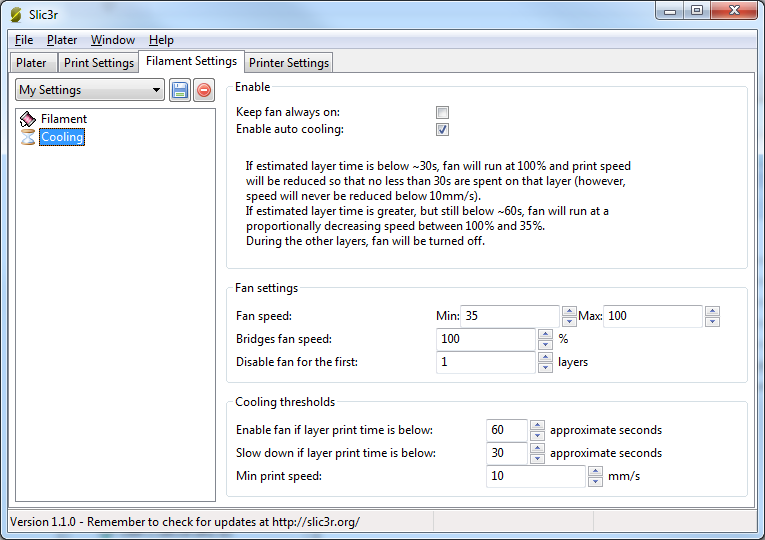
\includegraphics[keepaspectratio=true,width=1\textwidth]{expertmode/cooling_advanced_settings.png}
\caption{Param\`etres avanc\'es de refroidissement}
\label{fig:cooling_advanced_settings}
\end{figure}

\begin{itemize}
    \index{Filament Settings!Cooling!Cooling!Keep fan always on}
	\index{Param\`etres du Filament!Refroidissement!Garder le ventilateur allum\'e}
	\item \texttt{Keep Fan always on} (Garder le ventilateur allum\'e) - Si cette option est activ\'ee, le ventilateur ne sera jamais d\'esactiv\'ee et sera maintenu en marche au moins \`a sa vitesse minimum. Utile pour PLA, nuisible pour l'ABS.
    \index{Filament Settings!Cooling!Enable auto cooling}
	\index{Param\`etres du Filament!Refroidissement!Activer le refroidissement automatique}
	\item \texttt{Enable auto cooling} (Activer le refroidissement automatique) - Cela active / d\'esactive la logique de refroidissement. Un texte descriptif au dessous explique les effets de la configuration actuelle.
\end{itemize}


\begin{itemize}
    \index{Filament Settings!Cooling!Fan speed}
	\index{Param\`etres du Filament!Refroidissement!Vitesse du ventilateur}
	\item \texttt{Fan speed} (Vitesse du ventilateur) - D\'etermine la vitesse minimum et maximum - utile pour les ventilateurs qui vont trop vite par d\'efaut.
    \index{Filament Settings!Cooling!Bridges fan speed}
	\index{Param\`etres du Filament!Refroidissement!Vitesse du ventilateur pour les ponts}
	\item \texttt{Bridges fan speed} (Vitesse du ventilateur pour les ponts) - Comme la mati\`ere s'\'etire dans le vide sur de grands \'ecarts, il est logique d'essayer de la refroidir autant que possible, donc la vitesse maxi du ventilateur est recommand\'e.
    \index{Filament Settings!Cooling!Disable fan for first n layers}
	\index{Param\`etres du Filament!Refroidissement!D\'esactiver le ventilateur pour les n 1ere couches}
	\item \texttt{Disable fan for first \textit{n} layers} (D\'esactiver le ventilateur pour les \textit{n} 1ere couches) - La section \ref{sec:the_important_first_layer} montre l'importance de la premi\`ere couche , il est donc logique de ne pas appliquer le ventilateur jusqu'\`a ce que l'impression soit solidement fix\'e au lit. Garder le ventilateur \'eteint pendant les deux ou trois premi\`eres couches est une bonne id\'ee.
\end{itemize}

\begin{itemize}
    \index{Filament Settings!Cooling!Enable fan if print time is below t seconds}
	\index{Param\`etres du Filament!Refroidissement!Activer le ventilateur si temps d'impression inf\'erieur \`a t secondes}
	\item \texttt{Enable fan if print time is below \textit{t} seconds}  (Activer le ventilateur si temps d'impression inf\'erieur \`a \textit{t} secondes) - D\'eclenche le ventilateur, si la couche sera termin\'e dans le nombre donn\'e de secondes.
    \index{Filament Settings!Cooling!Slow down if layer print time is below t seconds}
	\index{Param\`etres du Filament!Refroidissement!Ralentir si temps d'impression inf\'erieur \`a t secondes}
	\item \texttt{Slow down if layer print time is below \textit{t} seconds}  (Ralentir si temps d'impression inf\'erieur \`a \textit{t} secondes) - Ralentit l'impression si la couche sera termin\'e dans le nombre donn\'e de secondes.
    \index{Filament Settings!Cooling!Min print speed}
	\index{Param\`etres du Filament!Refroidissement!Vitesse d'impression minimum}
	\item \texttt{Min print speed}  (Vitesse d'impression minimum) - Une limite inf\'erieure de la lenteur avec laquelle une couche peut \^etre imprim\'e.
\end{itemize}


% subsection configuring_cooling (end)

% section cooling (end)


\newpage

%!TEX root = Slic3r-Manual.tex
\section{Mati\`ere de Support} % (fold)
\label{sec:support}
\index{support material}
\index{mati\`ere de support}

En g\'en\'eral, la plupart des mod\`eles 3D seront imprim\'es avec des parties en surplomb jusqu'\`a une certaine inclinaison. L'angle est d\'etermin\'e par plusieurs facteurs, notamment la hauteur de la couche et la largeur d'extrusion, et est g\'en\'eralement autour de 45 °. Pour les mod\`eles avec de plus grands surplombs une structure de support peut \^etre imprim\'e en dessous. Cela engage l'utilisation de plus de mati\`ere, plus de temps d'impression, et un nettoyage apr\`es l'impression.

\begin{figure}[H]
\centering
\includegraphics[keepaspectratio=true,width=1\textwidth]{expertmode/support/advanced_support.png}
\caption{Param\`etres de support.}
\label{fig:advanced_support}
\end{figure}
\index{Print Settings!Support material!Generate support material}
\index{Param\`etres d'Impression!Mati\`ere de Support!G\'en\'erer un support}
\index{Print Settings!Support material!Overhang threshold}
\index{Param\`etres d'Impression!Mati\`ere de Support!Seuil de porte \`a faux}
\index{Print Settings!Support material!Enforce support}
\index{Param\`etres d'Impression!Mati\`ere de Support!Appliquer le support}

La premi\`ere chose \`a faire est d'activer l'option de mati\`ere de support en cochant la case \texttt{Generate support material} (G\'en\'erer un support).  Mettre \`a z\'ero le param\`etre \texttt{Overhang threshold} (Seuil de porte \`a faux) indique \`a Slic3r de d\'etecter les lieux o\`u apporter un soutien automatiquement, sinon l'angle indiqu\'e sera utilis\'e.  La g\'en\'eration de support est un sujet relativement complexe, et il y a plusieurs aspects qui d\'eterminent le soutien optimal, il est fortement recommand\'e de fixer le seuil \`a z\'ero et permettre Slic3r de d\'eterminer le soutien n\'ecessaire.

Les petits mod\`eles, et ceux avec de petites empreintes \`a la base, peuvent parfois se briser ou se d\'etacher du lit.  Pour cette raison le param\`etre \texttt{Enforce support} (Appliquer le support) produira des structures de support \`a imprimer pour le nombre donn\'e de couches, ind\'ependamment de la valeur de seuil d'angle.

Pour d\'emontrer les modes de remplissage le mod\`ele minimug a \'et\'e inclin\'e de 45 ° le long de l'axe x, comme repr\'esent\'e sur la figure \ref{fig:support_minimug_45deg}.
\index{Print Settings!Support material!Pattern}
\index{Param\`etres d'Impression!Mati\`ere de Support!Motif}

\begin{figure}[H]
\centering
\includegraphics[keepaspectratio=true,width=0.75\textwidth]{expertmode/support/support_minimug_45deg.png}
\caption{Mod\`ele Minimug, inclin\'e \`a 45°.}
\label{fig:support_minimug_45deg}
\end{figure}

Comme avec le remplissage, il existe plusieurs motifs disponibles pour la structure de support.

\begin{figure}[H]
\centering
\includegraphics[keepaspectratio=true,width=0.2\textwidth]{expertmode/support/support_pattern_rectlinear.png}
\caption{Motif de support: Rectiligne}
\label{fig:support_pattern_rectlinear}
\end{figure}

\begin{figure}[H]
\centering
\includegraphics[keepaspectratio=true,width=0.2\textwidth]{expertmode/support/support_pattern_rectlinear_grid.png}
\caption{Motif de support: Grille Rectiligne}
\label{fig:support_pattern_rectlinear_grid}
\end{figure}

\begin{figure}[H]
\centering
\includegraphics[keepaspectratio=true,width=0.2\textwidth]{expertmode/support/support_pattern_honeycomb.png}
\caption{Motif de support: Nid d'Abeille}
\label{fig:support_pattern_honeycomb}
\end{figure}
\index{Print Settings!Support material!Pattern Spacing}
\index{Param\`etres d'Impression!Mati\`ere de Support!Espacement du Motif}

\index{Print Settings!Support material!Pattern Angle}
\index{Param\`etres d'Impression!Mati\`ere de Support!Angle du Motif}

\texttt{Pattern Spacing} (Espacement du Motif) d\'etermine la distance entre les lignes de support, et est comparable \`a la densit\'e de remplissage en plus d'\^etre d\'efinie seulement en mm. Si vous changez cet attribut tenez compte de la largeur de l'extrusion du support et de la quantit\'e de mati\`ere de support qui adh\`ere \`a l'objet.

Il faut prendre soin de choisir un motif de support qui correspond au mod\`ele, o\`u le support se fixe perpendiculairement \`a la paroi de l'objet, plut\^ot que parall\`element, de sorte qu'il sera facile \`a retirer.  Si la structure de support court le long de la longueur d'une paroi alors le param\`etre \texttt{Pattern Angle} (Angle du Motif) permet la rotation de la direction des lignes de support

\begin{figure}[H]
\centering
\includegraphics[keepaspectratio=true,width=0.2\textwidth]{expertmode/support/support_pattern_rectlinear_rotated.png}
\caption{Exemple de motif tourn\'e \`a 45°.}
\label{fig:support_pattern_rectlinear_rotated}
\end{figure}


%TODO: Interface layers.


% section support (end)


\newpage

%!TEX root = Slic3r-Manual.tex

\section{Largeur d'Extrusion} % (fold)
\label{sec:extrusion_width}
\index{extrusion width}
\index{largeur d'extrusion}

\begin{figure}[H]
\centering
\includegraphics[keepaspectratio=true,width=1\textwidth]{expertmode/advanced_extrusion_widths_options.png}
\caption{Paramètres de largeur d'Extrusion.}
\label{fig:advanced_extrusion_widths_options}
\end{figure}

Une des raisons de la modification de la largeur de l'extrusion a déjà été examinée: l'augmentation de la largeur d'extrusion de la première couche dans le but d'améliorer l'adhesion au lit. (voir p.\pageref{par:wider_extrusion_width}).  Il y a quelques autres cas où il peut être bénéfique de modifier la largeur d'extrusion.
\begin{itemize}
    \item \texttt{Perimeter} (Périmètre) - Une valeur plus faible produira des extrusions minces qui à leurs tour produiront des surfaces plus précise.
    \item \texttt{Infill} (Remplissage) et \texttt{Solid Infill} (Remplissage solide) - Une extrusion épaisse pour le remplissage produira des impressions plus rapides et des pièces plus solides.
    \item \texttt{Top infill} (Remplissage suppérieur) - Une extrusion fine, améliorera la finition de la surface et assurera que les coins soient bien remplis.
    \item \texttt{Support material} (Matière de Support) - Comme avec les options de remplissage, une extrusion épaisse permettra de réduire le temps d'impression.
\end{itemize}

Il est important de se rappeler que, si la largeur de l'extrusion est exprimée en pourcentage, elle se calcule à partir de la propriété \texttt{Layer height} (Hauteur de couche), et non du paramètre \texttt{Default extrusion width} (Largeur d'extrusion par défaut).

% section extrusion_width (end)


\newpage

\input{SequentialPrinting}

\newpage

%!TEX root = Slic3r-Manual.tex

\section{Hauteur de couche variable} % (fold)
\label{sec:variable_layer_height}
\index{layer height}
\index{hauteur de couche}

Slic3r donne la possibilit\'e de r\'egler la hauteur de couche entre des positions arbitraires le long de l'axe Z. Voil\`a, des parties du mod\`ele peuvent \^etre imprim\'es avec une hauteur de couche grossi\`ere, par exemple des sections verticales, et d'autres parties pourraient \^etre imprim\'es avec une hauteur de couche plus fine, par exemple les d\'egrad\'es inclin\'es o\`u les couches apparaissent plus marqu\'ees.

Le mod\`ele de la fig. \ref{fig:example_model} donne un exemple rudimentaire o\`u des hauteurs de couche variables pourraient \^etre utilis\'ees pour am\'eliorer la qualit\'e d'impression.  Les murs de la structure n'ont pas \`a \^etre imprim\'es en haute d\'efinition pour une qualit\'e acceptable, mais la pente du toit apparait en escalier, une hauteur de couche de 0,4 mm est trop grossi\`ere, en particulier pour la couche sup\'erieure, qui est aplatie.  Ceci est illustr\'e dans le G-Code repr\'esent\'e \`a la fig \ref{fig:example_gcode_normal_layer_heights}.


\begin{figure}[H]
\centering
\includegraphics[keepaspectratio=true,width=0.75\textwidth]{expertmode/variable_layer_height/example_model.png}
\caption{Exemple de mod\`ele mettant en evidence un cas d'utilisation des couches variables.}
\label{fig:example_model}
\end{figure}

\begin{figure}[H]
\centering
\includegraphics[keepaspectratio=true,width=0.75\textwidth]{expertmode/variable_layer_height/example_gcode_normal_layer_heights.png}
\caption{Exemple avec des couches normales.}
\label{fig:example_gcode_normal_layer_heights}
\end{figure}

Les param\`etres de hauteur de couche variables sont disponibles en double-cliquant sur ​​le nom de la pi\`ece dans la fen\^etre Plater (surface de travail).  Cela ouvrira une fen\^etre qui contient deux onglets. Le premier donne des informations sur le mod\`ele, comme indiqu\'e dans la fig. \ref{fig:variable_layer_height_options_tab_1}.

\begin{figure}[H]
\centering
\includegraphics[keepaspectratio=true,width=0.75\textwidth]{expertmode/variable_layer_height/variable_layer_height_options_tab_1.png}
\caption{Param\`etres de Couche variable - Info.}
\label{fig:variable_layer_height_options_tab_1}
\end{figure}

Il convient de noter la hauteur du mod\`ele, puisque cela sera utile pour le calcul de la hauteur maximale de Z.

Le deuxi\`eme onglet (fig. \ref{fig:variable_layer_height_options_tab_2}) pr\'esente un tableau dans lequel chaque rang\'ee d\'efinit une hauteur de couche pour une plage particuli\`ere le long de l'axe Z, exprim\'ee en millim\`etres. Dans cet exemple, les parois du mod\`ele sont imprim\'ees \`a 0,4 mm, les parties raides du toit sont imprim\'ees \`a 0,2 mm, et la moins raide \`a 0,15 mm. Notez que chaque plage se divise exactement par la hauteur de la couche donn\'ee de sorte qu'il n'y a pas de «trous» entre les sections.

\begin{figure}[H]
\centering
\includegraphics[keepaspectratio=true,width=0.75\textwidth]{expertmode/variable_layer_height/variable_layer_height_options_tab_2.png}
\caption{Param\`etres de Couche variable - Layers (Couches).}
\label{fig:variable_layer_height_options_tab_2}
\end{figure}

Le G-Code r\'esultant (fig. \ref{fig:example_gcode_variable_layer_heights}) montre une plus haute d\'efinition qui devrait aboutir \`a une impression de qualit\'e sup\'erieure.

\begin{figure}[H]
\centering
\includegraphics[keepaspectratio=true,width=0.75\textwidth]{expertmode/variable_layer_height/example_gcode_variable_layer_heights.png}
\caption{Exemple avec une hauteur de couche variable.}
\label{fig:example_gcode_variable_layer_heights}
\end{figure}

La Fig. \ref{fig:example_print} montre le mod\`ele d'exemple imprim\'e.  L'impression de gauche a 0,4 mm  de hauteur de couche partout, alors que l'impression de droite a une hauteur de couche variable.

\begin{figure}[H]
\centering
\includegraphics[keepaspectratio=true,width=1\textwidth]{expertmode/variable_layer_height/example_print.jpg}
\caption{Exemple d'impression avec une hauteur de couches variable.}
\label{fig:example_print}
\end{figure}

Une caract\'eristique suppl\'ementaire de l'option de hauteur de couches variable est que par la saisie d'un z\'ero pour une plage de la partie du mod\`ele ne sera pas imprim\'e.  Fig. \ref{fig:example_gcode_skipped_layers} montre le G-Code o\`u des couches entre 0 et 4 mm sont ignor\'es. Il s'agit d'un moyen utile de diviser un grand mod\`ele en plusieurs sections plus courtes, qui peuvent \^etre imprim\'es individuellement et assembl\'es par la suite.
\begin{figure}[H]
\centering
\includegraphics[keepaspectratio=true,width=0.75\textwidth]{expertmode/variable_layer_height/example_gcode_skipped_layers.png}
\caption{Exemple avec des couches ignor\'ees.}
\label{fig:example_gcode_skipped_layers}
\end{figure}

% section variable_layer_height (end)

\newpage

%!TEX root = Slic3r-Manual.tex

Il y a deux façons d'organiser les param\`etres de configuration: exporter et importer les param\`etres de configuration, et des profils. Le premier est disponible en mode simple et expert, alors que les profils sont disponibles uniquement en mode expert.

\section{Export et Import de la Configuration} % (fold)
\label{sub:exporting_and_importing_configuration}
\index{configuration!export}
\index{configuration!import}

L'ensemble actuel d'options de configuration peut \^etre tout simplement export\'e via le menu File (Fichier)  \texttt{Export Config}. Cela permet se sauvegarder toutes les valeurs dans un fichier texte avec l'extention \texttt{.ini} .  Les fichiers pr\'ec\'edemment enregistr\'es peuvent \^etre charg\'es avec le menu File (Fichier) \texttt{Load Config} (charger la configuration).

Cela donne un des moyens rudimentaires pour stocker des param\`etres de configuration pour les diff\'erents besoins. Par exemple, un ensemble avec des vitesses d'impression l\'eg\`erement plus rapides, ou un motif de remplissage diff\'erent. Cependant, cette façon d'organiser les choses va vite devenir frustrante, car chaque changement mineur d'un param\`etre pourrait \^etre \`a dupliquer dans de nombreuses configurations. Pour cette raison, les profils sont de façon plus appropri\'ee de g\'erer plusieurs configurations.

Cette m\'ethode permet \'egalement le transfert de configurations entre machines, ou le stockage \`a distance.

% section exporting_and_importing_configuration (end)


\section{Profils} % (fold)
\label{sec:profiles}
\index{profiles}
\index{profils}

Apr\`es quelques impressions, il deviendra \'evident qu'il est utile d'avoir un ensemble d'options de configuration \`a choisir, et que certains param\`etres changent plus souvent que d'autres. En mode expert, des profils peuvent \^etre cr\'e\'es pour les param\`etres d'impression, de Filament et d'imprimante, dans l'espoir que les param\`etres d'imprimante changent peu souvent, de filaments rarement, cependant les param\`etres d'impression peuvent \^etre modifi\'es pour chaque mod\`ele. Ces diff\'erents profils peuvent \^etre m\'elang\'es et combin\'es \`a volont\'e, et peuvent \^etre s\'electionn\'es dans leurs onglets respectifs, ou directement \`a partir de la surface de travail.

\subsection{Cr\'eation des Profils} % (fold)
\label{sub:creating_profiles}
\index{profiles!create}
\index{profils!cr\'eer}

Ouvrez l'onglet souhait\'e et modifiez les param\`etres si n\'ecessaire. Une fois satisfait, cliquez sur l'ic\^one de sauvegarde vers la gauche au-dessus des titres de r\'eglage, et donner un nom appropri\'e \`a l'invite.

\begin{figure}[H]
\centering
\includegraphics[keepaspectratio=true,width=1\textwidth]{organising/creating_a_profile.png}
\caption{Sauver un profil.}
\label{fig:creating_a_profile}
\end{figure}

\index{profiles!delete}
\index{profils!effacer}
Les profils peuvent \^etre supprim\'es, en choisissant le profil \`a supprimer et en cliquant sur le bouton rouge supprimer \`a c\^ot\'e du bouton Enregistrer.

\begin{figure}[H]
\centering
\includegraphics[keepaspectratio=true,width=1\textwidth]{organising/deleting_a_profile.png}
\caption{Effacer un profil.}
\label{fig:deleting_a_profile}
\end{figure}

% subsection creating_profiles (end)


% section profiles (end)

}
\fi
%%% END EXPERT MODE %%%

%%% INPUT OUTPUT FILES %%%
\ifadvanced
\chapter{\emph{Fichiers d'entr\'es et de sorties}}
\thispagestyle{empty}
\markboth{Fichiers d'entr\'es et de sorties}{Manuel Utilisateur de Slic3r}
{%!TEX root = Slic3r-Manual.tex

%!TEX root = Slic3r-Manual.tex

Si le maillage 3D d\'ecrit dans le mod\`ele contient des trous, ou les bords ne sont pas align\'es (connu comme \'etant non-manifold), alors Slic3r peut avoir des probl\`emes de traitement . Slic3r va tenter de r\'esoudre les probl\`emes, s'il le peut, mais certains probl\`emes sont hors de sa port\'ee. Si l'application indique que le mod\`ele ne peut pas \^etre tranch\'e correctement alors il y a plusieurs options disponibles, et celles d\'ecrites ici sont toutes libres au moment de l'\'ecriture.

%%% CONFIGURATION TUNING %%%
{\input{WorkingWithModelsNetfabb}}
%%% END CONFIGURATION TUNING %%%

\paragraph{FreeCAD} % (fold)
\label{par:freecad}
\index{FreeCAD}

Freecad\footnote{\url{http://sourceforge.net/projects/free-cad}} est un logiciel de CAO, complet et gratuit, qui est livr\'e avec un module de maillage, dans lequel on peut effectuer les r\'eparations d'erreur dans les mod\`eles. Les \'etapes suivantes d\'ecrivent comment un probl\`eme dans un fichier de mod\`ele peut \^etre analys\'e et r\'epar\'e.

\begin{figure}[H]
\centering
\includegraphics[keepaspectratio=true,width=0.75\textwidth]{working_with_models/freecad_part_repair.png}
\caption{R\'eparation avec FreeCAD.}
\label{fig:freecad_part_repair}
\end{figure}

\begin{itemize}
	\item Lancer FreeCAD et \`a partir la page d'accueil choisir \texttt{Working with Meshes}.
	\item Chargez le mod\`ele en le faisant glisser sur l'espace de travail ou par l'interm\'ediaire du menu \texttt{File}.  Un petit message dans le coin en bas \`a gauche indique si le mod\`ele semble avoir des probl\`emes.
	\item Dans le menu choisissez \texttt{Meshes->Analyze->Evaluate \& Repair mesh} pour faire appara\^itre la bo\^ite de dialogue des options de r\'eparation.
	\item Dans la bo\^ite de dialogue choisir la maille charg\'ee, puis effectuer chaque analyse soit en cliquant sur le bouton \texttt{Analyze} par type de probl\`eme, ou s\'electionnez \texttt{Repetitive Repair} en bas pour effectuer tous les contr\^oles. Si un probl\`eme  correspondant est d\'etect\'e le bouton \texttt{Repair} devient actif.
	\item Pour chaque r\'eparation souhait\'e frapper le bouton \texttt{Repair}.
	\item Il est important d'examiner l'effet que le script de r\'eparation a apport\'e au mod\`ele.  Il se peut que le script produise des dommages dans le fichier, plut\^ot que de le r\'eparer, par exemple en retirant des triangles importants.
	\item Exporter le mod\`ele r\'epar\'e par le menu \texttt{Export} ou le menu contextuel.
\end{itemize}
% paragraph freecad (end)


\newpage

%!TEX root = Slic3r-Manual.tex

\section{Sortie SVG} % (fold)
\label{sec:svg_output}
\index{SVG}
\index{DLP resin printer}
\index{imprimante r\'esine DLP}
\index{powder-bed printer}
\index{imprimante \`a poudre}

Slic3r peut produire une sortie pour d'autres types d'imprimantes 3D qui n\'ecessitent que chaque couche soit repr\'esent\'e en image, par exemple les imprimante r\'esine DLP ou \`a poudre-lit. Ces imprimantes attendent une image g\'en\'eralement constitu\'e d'une silhouette blanche sur un fond noir (voir figure \ref{fig:example_svg_slice}).  Presque tous les formats d'image peuvent \^etre utilis\'es (bmp, png, etc), cependant, parce que l'image peut \^etre r\'eduite, il est g\'en\'eralement souhaitable d'utiliser un format vectoriel, plut\^ot qu'un format bitmap. Pour cette raison, il est courant d'utiliser le format "Scalable Vector Graphics" (SVG).

\begin{figure}[H]
\centering
\includegraphics[keepaspectratio=true,width=0.5\textwidth]{advanced/svg_output/example_svg_slice.png}
\caption{Exemple de tranche SVG.}
\label{fig:example_svg_slice}
\end{figure}

\index{Menu!Slice to SVG...}
\index{Menu!Trancher au format SVG...}

Slic3r offre la possibilit\'e de produire une sortie SVG appropri\'e pour de telles imprimantes.  Au lieu d'utiliser le \texttt{Plater}, le processus commence par la s\'election de l'option \texttt{Slice to SVG...} du menu \texttt{File}.  Celui-ci demande le fichier source (STL, OBJ ou AMF), et lorsqu'il est s\'electionn\'e demande o\`u le fichier SVG de sortie doit \^etre enregistr\'e. Ensuite Slic3r d\'emarre et produit le fichier SVG.

Tenter de voir le fichier SVG dans un navigateur entra\^inera seulement l'affichage de la premi\`ere couche, et seules les \^iles n\'egatifs dans le mod\`ele (comme l'arri\`ere-plan du navigateur est g\'en\'eralement blanc).

\begin{figure}[H]
\centering
\includegraphics[keepaspectratio=true,width=0.75\textwidth]{advanced/svg_output/svg_direct_browser.png}
\caption{le fichier SVG vu dans un navigateur.}
\label{fig:svg_direct_browser}
\end{figure}

Pour cette raison, une petite application web a \'et\'e \'ecrite pour permettre de visualiser chaque tranche sur un fond noir\footnote{\url{http://garyhodgson.github.io/slic3rsvgviewer}}.  Acc\'edez \`a l'application et faites glisser le fichier SVG sur l'\'ecran pour le charger et l'afficher.

\begin{figure}[H]
\centering
\includegraphics[keepaspectratio=true,width=0.75\textwidth]{advanced/svg_output/svg_slic3rsvg_viewer.png}
\caption{Slic3r SVG Viewer.}
\label{fig:svg_slic3rsvg_viewer}
\end{figure}

\subsection{Param\`etres SVG} % (fold)
\label{sub:svg_settings}

La majorit\'e des options dans Slic3r ne sont pas n\'ecessaires pour la g\'en\'eration SVG, cependant le param\`etre \texttt{Layer height} d\'eterminera le nombre de couches. Notez que Slic3r limite la hauteur de la couche pour qu'elle soit plus petite que le diam\`etre de la buse, donc cela peut \'egalement \^etre augmenter si l'on souhaite des couches plus hautes.

% subsection svg_settings (end)

\subsection{Imprimer \`a partir de fichiers SVG} % (fold)
\label{sub:printing_with_svg}

Alors que la sortie SVG peut \^etre utilis\'e pour une gamme d'imprimantes, l'exemple suivant montre comment le fichier, peut \^etre utilis\'e avec une imprimante r\'esine DLP. En utilisant une version modifi\'ee de Printrun \footnote{\url{http://garyhodgson.com/reprap/projectlayer}} le fichier SVG peut \^etre charg\'e directement et envoy\'e \`a un projecteur DLP. L'axe Z est contr\^ol\'ee par des commandes G-code envoy\'e par le composant printcore, ce qui signifie que l'\'electronique RepRap standard, tels que RAMPS, peuvent \^etre utilis\'es.


\begin{figure}[H]
\centering
\includegraphics[keepaspectratio=true,width=0.75\textwidth]{advanced/svg_output/projectlayer.png}
\caption{Impression SVG avec Projectlayer.}
\label{fig:projectlayer}
\end{figure}


% subsection printing_with_svg (end)

% section svg_output (end)

}
\fi
%%% END INPUT OUTPUT FILES %%%

%%% ADVANCED %%%
\ifadvanced
\chapter{\emph{Sujets Avanc\'es}}
\thispagestyle{empty}
\markboth{Sujets Avanc\'es}{Manuel Utilisateur de Slic3r}
{%!TEX root = Slic3r-Manual.tex

%!TEX root = Slic3r-Manual.tex

\section{Extrudeuse Multiple} % (fold)
\label{sec:multiple_extruders}
\index{extruders!multiple}
\index{extrudeuse!multiple}

Une imprimante avec plus d'une extrudeuse peut \^etre utilis\'e de diff\'erentes mani\`eres. Si vous avez un modèle multi-partie, qui définit des régions distinctes, vous pouvez assigner chacun d'eux à une extrudeuse. Si vous avez un modèle de pièce unique, vous pouvez attribuer des rôles différents à chaque extrudeuse: par exemple, vous pouvez remblayer l'aide d'une grosse buse ou vous pouvez construire matériau support avec filament soluble


\subsection{Configurer les Extrudeuses} % (fold)
\label{sub:configuring_extruders}
\index{Printer Settings!General!Capabilities!Extruders}
\index{Param\`etres de l'Imprimante!Fonctionnalit\'es!Extrudeuses}

Dans l'onglet \texttt{Printer Settings} (Param\`etres de l'Imprimante) il y a le param\`etre \texttt{Extruders} (Extrudeuses), dans la section \texttt{Capabilities} (Fonctionnalit\'es), ce qui permet de d\'efinir le nombre d'extrudeuses. Incr\'ementer cette valeur ajouter dynamiquement une autre d\'efinition d'extrudeuse dans le volet de gauche.

\begin{figure}[H]
\centering
\includegraphics[keepaspectratio=true,width=1\textwidth]{expertmode/multipleextruders/printer_settings_general_multiple_extruder_options.png}
\caption{Param\`etres d'Extrudeuses Multiples - Onglet Param\`etre de l'Imprimante (G\'en\'eral).  Notez les deux extrudeuses d\'efinies dans le volet de gauche.}
\label{fig:printer_settings_general_multiple_extruder_options}
\end{figure}

Chaque extrudeuse peut \^etre configur\'e comme d'habitude, mais il y a d'autres param\`etres qui doivent \^etre d\'efinis qui sont notamment les configurations multi-extrudeuse.

\begin{figure}[H]
\centering
\includegraphics[keepaspectratio=true,width=1\textwidth]{expertmode/multipleextruders/printer_settings_extruder_multiple_extruder_options.png}
\caption{Param\`etres d'Extrudeuses Multiples - Onglet Param\`etre de l'Imprimante (Extruder).}
\label{fig:printer_settings_extruder_multiple_extruder_options}
\end{figure}

\index{Printer Settings!Extruder!Extruder offset}
\index{Param\`etres de l'Imprimante!D\'ecalage de l'extrudeuse}

l'\texttt{Extruder offset} (D\'ecalage de l'extrudeuse) doit \^etre utilis\'e si le microprogramme ne g\`ere pas le d\'ecalage de chaque buse suppl\'ementaire. La documentation de votre micrologiciel devrait vous dire si c'est le cas. Chaque extrudeuse suppl\'ementaire a un d\'ecalage par rapport \`a la premi\`ere (qui a généralement 0,0). Si le firmware le g\`ere, toutes les compensations peuvent rester \`a 0,0.

\index{Printer Settings!Extruder!Retraction!Length}
\index{Param\`etres de l'Imprimante!Extrudeuse!R\'etractation!Longueur}
Parce que l'extrudeuse secondaire sera en sommeil tandis que la premi\`ere est cours d'utilisation, et vice-versa, il est important que le mat\'eriau soit suffisamment r\'etract\'e pour cesser le suintement.  Comme avec les r\'eglages ordinaires de r\'etractation (voir p. \pageref{fig:retraction_settings}) le param\`etre \texttt{Length} (Longueur) est mesur\'e \`a partir du filament entrant dans l'extrudeuse.

% subsection configuring_extruders (end)

\subsection{Attribution de filaments} % (fold)
\label{sub:assigning_filaments}
\index{Plater}
\index{Surface de Travail}
Quand un profil d'imprimante avec plusieurs extrudeuses a \'et\'e s\'electionn\'e, l'onglet \texttt{Plater} (Surface de Travail) permet la s\'election d'un filament diff\'erent pour chaque extrudeuse.

\begin{figure}[H]
\centering
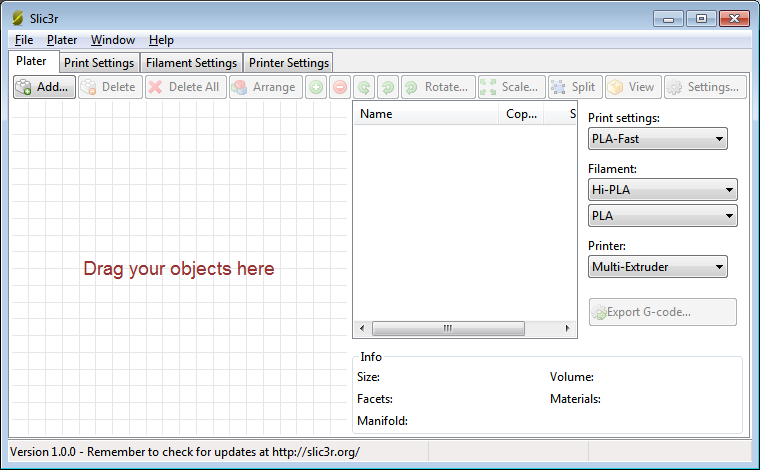
\includegraphics[keepaspectratio=true,width=1\textwidth]{expertmode/multipleextruders/plater_multi_filament.png}
\caption{Surface de travail avec de multiple param\`etre de filaments.}
\label{fig:plater_multi_filament}
\end{figure}

% subsection assigning_filaments (end)

\subsection{Affectation des extrudeuses pour les objets mono-mati\`ere} % (fold)
\label{sub:assigning_extruders}
\index{Print Settings!Multiple Extruders}
\index{Param\`etres de l'Imprimante!Extrudeuse Multiple}

Pour les impressions de mat\'eriaux unique, o\`u l'extrudeuse secondaire a pour mission une extrusion particuliere, la section \texttt{Multiple Extruders} (Extrudeuses multiples) de l'onglet \texttt{Print Settings} (Param\`etres de l'imprimante) donne la possibilit\'e d'assigner une extrudeuse pour chaque type d'extrusion.

\begin{figure}[H]
\centering
\includegraphics[keepaspectratio=true,width=1\textwidth]{expertmode/multipleextruders/print_settings_multiple_extruder_options.png}
\caption{Param\`etres d'Extrudeuse Multiple - Onglet Param\`etre d'Impression.}
\label{fig:advanced_multiple_extruder_options}
\end{figure}

% subsection assigning_extruders (end)

\subsection{Configurer le Changement d'Outil} % (fold)
\label{sub:configuring_tool_changes}

\index{Printer Settings!Custom G-code!Tool change G-code}
\index{Param\`etres de l'Imprimante!G-code personnalis\'e!G-code de changement d'outil}

La section \texttt{Custom G-code} (G-code personnalis\'e) de l'onglet \texttt{Printer Settings} (Param\`etres de l'Imprimante) dispose d'une option d'insertion de G-code entre les changements d'outils. Comme avec toutes les sections personnalis\'e G-code, les variables d'environement peuvent \^etre utilis\'ees afin de r\'ef\'erencer les param\`etres Slic3r.  Cela inclus les variables [previous\_extruder] et [next\_extruder].

\begin{figure}[H]
\centering
\includegraphics[keepaspectratio=true,width=1\textwidth]{expertmode/multipleextruders/printer_settings_custom_gcode.png}
\caption{Param\`etres d'Extrudeuse Multiple - G-code de Changement d'outil.}
\label{fig:printer_settings_custom_gcode}
\end{figure}

% subsection configuring_tool_changes (end)


\subsection{Impression d'objets multi-mati\`eres} % (fold)
\label{sub:printing_multi_material_objects}

Si un fichier multi-mat\'eriaux AMF existe d\'ej\`a, parce que le programme de CAO peut exporter un tel format, alors celui-ci peut \^etre charg\'e dans Slic3r de façon habituelle. Le mappage entre mati\`eres de l'objet et les extrudeuses est s\'equentielle, c'est \`a dire que la premiere mati\`ere est affect\'e \`a la premi\`ere extrudeuse, etc.

% subsection printing_multi_material_objects (end)


\subsection{G\'en\'eration de fichiers AMF multi-mati\`ere} % (fold)
\label{sub:generating_multi_material_amf_files}

Slic3r a la capacit\'e de combiner plusieurs fichiers STL dans un fichier multi-mati\`ere AMF.

\index{Menu!Combine multi-material STL files...}
\index{Menu!Combiner des fichiers STL multi-mati\`ere...}

\begin{itemize}
    \item Diviser la conception originale dans les diff\'erentes parties au sein du programme de CAO, et exporter chaque partie en STL.
    \item Dans Slic3r, choisissez \texttt{Combine multi-material STL files...} (Combiner des fichiers STL multi-mati\`ere...) \`a partir du menu \texttt{File} (Fichier).
    \item Lorsque vous \^etes invit\'e avec une bo\^ite de dialogueChoisissez le premier STL, qui sera attribu\'e \`a la premi\`ere mati\`ere (et donc la premi\`ere extrudeuse). Cliquez sur \texttt{Open} pour \^etre invit\'e au prochain STL, et ainsi de suite jusqu'\`a ce que chaque STL soit affect\'es \`a une mati\`ere. Pour signaler qu'il n'y a plus de fichiers STL, choisissez \texttt{Cancel} (Annuler).
    \item La bo\^ite de dialogue suivante demande l'emplacement et le nom du fichier de l'AMF.
\end{itemize}

Une fois g\'en\'er\'e le fichier peut \^etre charg\'e et imprim\'e comme d\'ecrit ci-dessus.

% subsection generating_multi_material_amf_files (end)

% section multipe_extruders (end)


\newpage

\section{Qualit\'e Brouillon}

Plusieurs options peuvent être désactivées ou accordées afin d'obtenir une vitesse de génération de code G plus rapide et des temps d'impression plus courts.

\subsection{Print Settings \textgreater Layers and perimeters \textgreater Quality}

\begin{figure}[H]
\centering
\includegraphics[keepaspectratio=true,width=1\textwidth]{advanced/draft_quality_options.png}
\caption{Option de Qualit\'e}
\label{fig:draft_quality}
\end{figure}

Ces options fournissent des objets plus agréables et plus propres, mais nécessitent plus de temps CPU. Elles peuvent être désactivées pour les impressions en mode broullion.

\begin{itemize}
\item \texttt{Extra perimeters if needed} Cette fonctionnalité vérifie si l'ajout de paramètres à des couches en pente aiderait à masquer le remplissage interne, ce qui rend l'objet plus agréable.
\item \texttt{Avoid crossing perimeters:} Cette fonctionnalité mélange les déplacements afin que la buse reste à l'intérieur ou à l'extérieur de l'objet chaque fois que possible, ce qui réduit le nombre de fois qu'elle traverse les périmètres et déclenche une rétraction. Cela empêche la mise en chaîne mais nécessite beaucoup de temps CPU pendant l'exportation de code G car des algorithmes complexes de planification de mouvement sont utilisés pour chaque couche unique.
\item \texttt{Detect thin walls:} Cette fonctionnalité vérifie les collisions entre les périmètres. Il garantit que l'imprimante n'essaie pas d'extruder des chemins trop rapprochés et utilise l'algorithme de l'axe médian pour transformer des parois minces en extrusions à simple passage.
\item \texttt{Detect bridging perimeters:} Cette caractéristique détecte les portions de pont / surplomb des périmètres et leur applique le débit / vitesse de pont.
\end{itemize}

\subsection{Print Settings \textgreater Infill}

Lesmotifs de remplissage \textit{Hilbert Curve}, \textit{Archimedean Chords} et \textit{Octagram Spiral} sont généralement beaucoup plus lents. Vous pourriez vouloir les éviter dans vos tirages de qualité d'ébauche si vous vous souciez de la vitesse de découpage.

\subsection{Print Settings \textgreater Advanced \textgreater Resolution}

Par défaut, Slic3r ne simplifie pas la géométrie d'entrée et rendra tous les détails dans le G-code de sortie pour une précision maximale. Cependant, les modèles à haute résolution portent souvent plus de résolution que l'imprimante est capable d'imprimer, de sorte qu'ils peuvent être simplifiés, surtout lorsque vous voulez un découpage plus rapide. Vous pouvez définir l'option de résolution à quelque chose comme 0,05 mm ou même 0,1 mm pour vos tirages de qualité de tirage.

\subsection{Print settings \textgreater Advanced \textgreater Threads}

(Cet indice s'applique à tous les types d'impressions, pas seulement à la qualité du trait.) De nombreux algorithmes dans Slic3r supportent la parallélisation en utilisant plusieurs threads. Vous devez définir cette option sur le nombre de processeurs ou de noyaux de votre ordinateur.


\newpage

\input{CommandLineUsage}

\newpage

%!TEX root = Slic3r-Manual.tex

\section{Scripts de post-traitement} % (fold)
\label{sec:post_processing_scripts}
\index{scripts}
\index{post processing}
\index{post-traitement}

Il peut y avoir des moments o\`u le G-Code g\'en\'er\'e par Slic3r doit \^etre modifi\'e ou modifi\'e apr\`es qu'il ai \'et\'e cr\'e\'e. Pour cette raison, il existe la possibilit\'e d'ex\'ecuter des scripts dans le cadre des derni\`eres \'etapes dans le processus de tranchage\footnote{\url{https://github.com/alexrj/Slic3r/wiki/Writing-post-processing-scripts}}.

\index{Print Settings!Output options!Post-processing scripts}
\index{Param\`etres d'Impression!Param\`etres de sortie!Scripts de post-traitement}
Dans la section \texttt{Output options} (param\`etres de sortie) de l'onglet \texttt{Print Settings} (Param\`etres d'Impression), se trouve l'option \texttt{Post-processing scripts} (Scripts de post-traitement).  Le chemin d'acc\`es absolu de chaque script peut \^etre ajout\'e, s\'epar\'e par des points-virgules. Chaque script doit \^etre reconnu par le syst\`eme h\^ote et \^etre ex\'ecutable.

\begin{figure}[H]
\centering
\includegraphics[keepaspectratio=true,width=1\textwidth]{advanced/post_processing_scripts/post_processing_scripts_options.png}
\caption{L'option script de post-traitement.}
\label{fig:post_processing_scripts_options}
\end{figure}

Chaque script sera pass\'e par le chemin absolu du fichier G-code que Slic3r g\'en\`ere. Toutes les options de configuration Slic3r sont mises \`a la disposition des scripts par des variables d'environnement.  Ils commencent tous par \texttt{SLIC3R\_}.  Le script suivant \'ecrira toutes les options Slic3r sur la sortie standard:

\begin{figure}[H]
\small
\begin{verbatim}
        #!/bin/sh
        echo "Post-processing G-code file: $*"
        env | grep ^SLIC3R
\end{verbatim}
\caption{Exemple de script de post-traitement qui affiche les variables d'environment Slic3r.}
\label{fig:exaple_post_processing_script_env_vars}
\end{figure}

Des exemples de scripts peuvent \^etre trouv\'es dans le d\'ep\^ot GitHub\footnote{\url{https://github.com/alexrj/Slic3r/tree/master/utils/post-processing}}.


le mode "Perl's in-place" (\texttt{perl -i})facilite la modification du contenu du fichier G-code, sans avoir \`a copier, modifier et remplacer l'original. L'exemple suivant va simplement afficher le contenu sur la sortie standard:

\begin{figure}[H]
\small
\begin{verbatim}
        #!/usr/bin/perl -i
        use strict;
        use warnings;

        while (<>) {
             # modify $_ here before printing
             print;
        }
\end{verbatim}
\caption{Exemple de script de post-traitement qui affiche chaque ligne sur la sortie standard.}
\label{fig:exaple_post_processing_script_print_lines}
\end{figure}

% section post_processing_scripts (end)


\newpage

%!TEX root = Slic3r-Manual.tex

\section{Calcul des flux} % (fold)
\label{sec:flow_math}
\index{flow math}
\index{Calcul des flux}

Cette page explique les calculs utilis\'ees dans Slic3r pour d\'eterminer la quantit\'e de flux. La documentation sert de r\'ef\'erence, car il pourrait être utile d'essayer de meilleurs mod\`eles.

\subsection{Comprendre la largeur d'extrusion} % (fold)

Deux questions principales affectent le travail de Slic3r:
\begin{itemize}
\item \textbf{A quelle distance} les chemins d'extrusion doivent-ils être positionn\'es pour obtenir une finition r\'eguli\`ere?
\item \textbf{Quelle quantit\'e de mati\`ere} doit être extrud\'ee le long de ces chemins?
\end{itemize}

Si deux chemins adjacents sont \textbf{trop proches} (ou \textbf{trop de mati\`ere} est extrud\'ee), ils se chevauchent. Si deux chemins adjacents sont \textbf{trop \'eloign\'es} (ou si \textbf{le mat\'eriau est insuffisamment extrud\'e}), des interstices seront visibles et / ou les extrusions se d\'etacheront en raison d'une liaison insuffisante.

En extrudant plus ou moins tout en se d\'eplaçant (c'est-\`a-dire en changeant \textbf{le rapport vitesse de flux/vitesse tête}), on peut faire des chemins plus \'epais ou plus minces:

\begin{figure}[H]
\centering
\includegraphics[keepaspectratio=true,width=0.5\textwidth]{advanced/flow_math/extrusion_width.png}
\caption{Largeur d'extrusion}
\label{fig:extrusion_width}
\end{figure}

\textbf{Des chemins plus \'epais} auront \textbf{une meilleure liaison} avec la couche inf\'erieure, ce qui est bon pour les pi\`eces m\'ecaniques. Cependant, ils seront moins en mesure de rapprocher la forme de l'objet et de combler de minuscules lacunes ou des courbes \'etroites (pensez \`a un foret: un plus grand ne sera pas en mesure d'entrer dans des endroits \'etroits). Au contraire, \textbf{des chemins plus minces} fourniront moins de collage mais une meilleure pr\'ecision de forme.

Noter cependant que la largeur d'extrusion ne peut être contrôl\'ee que lors de l'extrusion sur une surface existante (telle qu'une couche pr\'ec\'edente ou un lit d'impression). Si on extrude \texttt{\`a l'air libre} (c'est-\`a-dire en pontage), la forme r\'esultante sera toujours \textbf{ronde} et \'egale au \textbf{diam\`etre de la buse}:

\begin{figure}[H]
\centering
\includegraphics[keepaspectratio=true,width=0.5\textwidth]{advanced/flow_math/bridge.png}
\caption{Section d'un pont}
\label{fig:bridge}
\end{figure}

En fait, si vous r\'eduisez le flux de mati\`ere, vous obtiendrez des cercles plus petits dans une certaine mesure, jusqu'\`a ce que la viscosit\'e plastique d\'ecide qu'il est temps de briser votre pont en raison de trop de tension. Si, au contraire, vous extrudez trop de mat\'eriau, la forme du filament extrud\'e ne changera pas (toujours \'egale au diam\`etre de la buse), mais vous obtiendrez un pont distandu.

Alors, partons d'une d\'efinition:

La largeur d'extrusion est \textbf{l'\'epaisseur d'un seul filament} extrud\'e soit \`a l'air libre, soit au-dessus d'une surface. Ce n'est \textbf{pas} la distance de deux chemins adjacents car un chevauchement sera g\'en\'eralement appliqu\'e afin d'obtenir une meilleure liaison.

\subsection{Ponts: le cas facile} % (fold)

Comme indiqu\'e ci-dessus, il n'y a qu'un seul d\'ebit correct pour le pontage: celui qui ne fait pas que votre pont s'affaisse ou se casse. Les extrusions sont \textbf{rondes} et leur \textbf{diam\`etre est \'egal au diam\`etre de la buse}. Des trajets parall\`eles seront positionn\'es de telle sorte qu'ils soient \textbf{tangents}, ainsi l'espacement entre un chemin et son voisin est \'egal au diam\`etre de la buse aussi. (Dans le cas des ponts, nous ne voulons pas de chevauchement car il a prouv\'e de tra\^iner les chemins existants.)

Le volume de mati\`ere requis pour un trajet de longueur unitaire est calcul\'e en cons\'equence \`a la forme cylindrique, donc avec une section transversale circulaire:

$E = (diametre buse/2)^2 * pi$

\subsection{Extrusion sur une surface} % (fold)

Dans ce cas le probl\`eme est: \texttt{quelle forme} notre extrusion obtenir? Nous savons qu'il sera \'ecras\'e horizontalement, mais aura-t-il une forme rectangulaire ou ovale? Quelle est la largeur d'extrusion maximale que nous pouvons obtenir avec un diam\`etre de buse donn\'e avant que le plastique commence \`a se recourber sur les côt\'es?

Slic3r suppose que la forme en coupe transversale d'une extrusion est un rectangle \`a extr\'emit\'es semi-circulaires. Ainsi, la relation entre la largeur et le volume d'extrusion souhait\'es pour extruder est la suivante:

\begin{figure}[H]
\centering
\includegraphics[keepaspectratio=true,width=0.5\textwidth]{advanced/flow_math/area1.png}
\caption{coupe transversale de l'extrusion}
\label{fig:area1}
\end{figure}

Lorsque la largeur d'extrusion de la cible est plus fine que la hauteur de la couche, la forme est impr\'evisible, nous utilisons simplement la même formule rectangulaire mais d\'ecourager l'utilisation de telles valeurs d'extrusion minces.

La formule ci-dessus fournit une fonction qui corr\`ele la largeur d'extrusion cible avec la quantit\'e de mati\`ere \`a extruder par unit\'e de distance:

$E = f(largeur extrusion, hauteur couche)$

\subsection{Espacement des passage} % (fold)

Bon, maintenant nous savons combien extruder pour faire un seul chemin de la largeur d\'esir\'ee. Mais \textbf{\`a quel point devrions-nous chevaucher} des chemins afin d'obtenir une liaison parfaite?

En supposant qu'il n'y ait pas de chevauchement, donc de trajectoires tangentes, il y aurait un espace vide (jaune):

\begin{figure}[H]
\centering
\includegraphics[keepaspectratio=true,width=0.5\textwidth]{advanced/flow_math/tangent.png}
\caption{coupe transversale de l'extrusion}
\label{fig:tangent}
\end{figure}

La section transversale de ces vides est g\'en\'eralement:

$aire vide = hauteur couche^2 - (hauteur couche/2)^2 * pi$

Id\'ealement, nous voudrions remplir toute cette zone jaune en plaçant les extrusions ferm\'ees les unes aux autres. Cependant, il est tr\`es peu probable que la seconde extrusion remplisse l'espace sous la pr\'ec\'edente, il y aurait donc un peu de vide. Le chevauchement id\'eal serait quelque chose comme:


$0 < facteur de recouvrement*aire vide < aire vide$


Avec \texttt{facteur de recouvrement} allant de 0 \`a 1. \texttt{facteur de recouvrement} repr\'esente la quantit\'e de vide restant entre les extrusions. Il est difficile d'estimer cette quantit\'e, car elle d\'epend probablement aussi de la viscosit\'e du plastique, de la vitesse d'extrusion et de la temp\'erature. Dans le pass\'e, plusieurs valeurs ont \'et\'e essay\'ees pour \texttt{facteur de recouvrement}, mais certains utilisateurs signalaient des chemins trop clairsem\'es. Une valeur de 1 est actuellement utilis\'ee pour garantir que l'erreur (qui est toujours pr\'esente) est enti\`erement du côt\'e de l'extrusion abondante plutôt que manquante de mati\`ere.

L'espacement des chemins est donc:

$espacement = largeur extrusion - hauteur couche * (1 - pi/4)$

\subsection{Valeur par d\'efaut} % (fold)

Slic3r permet aux utilisateurs de d\'efinir manuellement la largeur d'extrusion pour chaque type d'extrusion (p\'erim\`etres, remplissage, support, etc.) mais calcule les valeurs par d\'efaut si aucune valeur personnalis\'ee n'est saisie.

Pour la boucle ext\'erieure des p\'erim\`etres (alias p\'erim\`etres externes), Slic3r adoptera par d\'efaut une largeur d'extrusion mince, \'egale au diam\`etre de la buse * 1,05. Ceci est consid\'er\'e comme la plus fine largeur d'extrusion. Une largeur d'extrusion mince donne une \textbf{meilleure pr\'ecision} de la forme de l'objet et minimise les erreurs d'\'ecoulement caus\'ees par un filament irr\'egulier.

La largeur d'extrusion pour les autres passage est calcul\'ee en obtenant la section transversale du diam\`etre de buse configur\'e et en calculant ensuite la largeur d'extrusion produite par extrusion de cette quantit\'e de mat\'eriau. En d'autres termes, en \textbf{adaptant la vitesse d'\'ecoulement et la vitesse de la tête}. Le but de cette logique est de trouver le flux "natif" qui minimise les forces lat\'erales lors de l'extrusion. Une telle extrusion calcul\'ee est plafonn\'ee \`a une valeur maximale \'egale au diam\`etre de tuy\`ere * 1,7, \`a l'exception du remplissage interm\'ediaire interne où l'\'ecoulement natif complet est utilis\'e.


% section flow-math (end)


\newpage}
\fi
%%% END ADVANCED %%%

%%% TROUBLESHOOTING %%%
\ifadvanced
\chapter{\emph{D\'epannage}}
\thispagestyle{empty}
\markboth{D\'epannage}{Manuel Utilisateur de Slic3r}
{%!TEX root = Slic3r-Manual.tex

\section{Erreurs de dimension}

Si vous n'êtes pas satisfait de la précision dimensionnelle de vos impressions, vérifiez d'abord que votre microprogramme est correctement configuré: les échelons / millimètres pour les axes X, Y et Z doivent être calculés en fonction de vos courroies, poulies et vis filetées. Veuillez ne pas calibrer par essai et erreur: ces valeurs doivent être exactes. Utilisez la calculatrice de Josef Prusa\footnote{\url{http://www.prusaprinters.org/calculator/}}.

\subsection{Dimensions verticales}

Si vos dimensions verticales sont fausses (c'est-à-dire le long de l'axe Z) - et votre objet est généralement plus court que prévu - cela signifie que votre buse est trop basse, donc la première couche est trop pressée sur le lit d'impression. Pour résoudre ce problème, vous voudrez peut-être augmenter votre Z-endstop ou augmenter l'option de décalage Z dans Slic3r.

\subsection{Dimensions horizontales}

Le problème habituel est que les trous sont trop petits. Cela affecte habituellement uniquement les trous sur le plan horizontal (XY). Il y a plusieurs raisons à cela. Voyons les voir un par un:

\subsection{Rétrécissement du plastique}

Le plastique \textbf{rétrécit lors du refroidissement}. Différents types de plastique présentent un retrait différent, qui peut également dépendre de la température. Du fait de ce retrait, des trous circulaires (ou polygonaux) posés par l'extrudeuse au diamètre nominal finiront par diminuer après refroidissement.

\subsection{Plus de matière déposé à l'interieur}

Lorsque vous extrudez le long d'une courbe, plus de matériau par unité de distance est déposé dans le côté concave. Un tel matériau excessif rend le rayon interne plus court. Un algorithme de compensation a été proposé par Adrian Bowyer et il a été implémenté dans Slic3r il ya quelque temps, mais de nombreux utilisateurs se sont plaints de trous trop grands - il a été enlevé par la suite depuis plus petits trous sont meilleurs que les trous plus grands car ils peuvent être forés.

\subsection{Les courbes sont approximées par des polygones}

Les fichiers STL ne contiennent que des mailles composées de triangles plats, de sorte que ses sections planes ne peuvent contenir que des formes polygonales. Par exemple, un trou circulaire est approximé par un polygone:

\begin{figure}[H]
\centering
\includegraphics[keepaspectratio=true,width=0.3\textwidth]{troubleshooting/polygonal-hole.png}
\caption{Trou en forme de polygone}
\label{fig:polygonal-hole}
\end{figure}
Augmenter le nombre de segments dans votre CAO avant d'exporter le fichier STL aidera à réduire l'erreur. Les utilisateurs d'OpenSCAD peuvent vouloir utiliser la fonction polyhole () développée par nophead qui calcule le nombre optimal de segments.

\subsection{Le filament tend à couper les coins}

Puisque les courbes sont approximées par des polygones, il y a des sommets tranchants à leurs sommets. Cependant, le plastique tend à faire des coins arrondis, réduisant ainsi la zone interne du trou encore plus.

\subsection{Ondulation verticale}

Même si la précision dimensionnelle d'une seule couche était correcte, plusieurs couches empilées pourraient rendre le trou plus petit si elles ne sont pas exactement alignées. Les ondulation verticale (\ref{sec:z_wobble}) causée par des problèmes mécaniques réduira la taille des trous à l'enveloppe interne des couches empilées:

\begin{figure}[H]
\centering
\includegraphics[keepaspectratio=true,width=1\textwidth]{troubleshooting/z-wobble.png}
\caption{Ondulation verticale}
\label{fig:z_wobble}
\end{figure}

\subsection{Filament irrégulier}

Les filaments de qualité médiocre et de faible qualité n'ont pas un diamètre très régulier. Si vous mesurez leur diamètre le long d'un seul mètre d'entre eux, vous trouverez souvent de nombreuses valeurs différentes (et de nombreux filaments de mauvaise qualité et n'ont pas de section parfaitement ronde). Cette variation continue de diamètre produira un écoulement irrégulier et le trou résultant sera toujours l'enveloppe interne de toutes les couches:

\begin{figure}[H]
\centering
\includegraphics[keepaspectratio=true,width=1\textwidth]{troubleshooting/irregular-filament.png}
\caption{Filament irrégulier}
\label{fig:irregular_filament}
\end{figure}

\subsection{Contrecoup}

Le jeu est un défaut mécanique d'un ou plusieurs axes qui réduit essentiellement la quantité de mouvement réel chaque fois qu'un moteur inverse sa direction de rotation. Il est généralement causé par des ceintures lâches. Sur les imprimantes à lit mobile, son axe (habituellement Y) est plus sujet à un jeu à cause de l'inertie. Donc, si vous obtenez des erreurs de dimension différentes dans X et Y, cela est causé par le jeu. Vous aurez besoin de serrer votre ceinture. Aucun hack logiciel ne peut raisonnablement compenser une imprimante mal assemblée.

\subsection{Calcul de flux}

Bon, toutes les causes ci-dessus ne dépendent pas de Slic3r et, quand cela est possible, ils doivent être corrigés avant de tenter une solution logicielle.

Cela dit, les calculs de flux utilisés dans Slic3r jouent un bon rôle dans la prise des dimensions correctes, car il essaie de deviner quelle est la forme du matériau extrudé sera et comment l'épaisseur de l'extrusion résultera sur le plan horizontal donné une quantité de matériau. Étant une approximation, elle porte une erreur. La façon habituelle de traiter ces questions implique de régler le paramètre Extrusion Multiplier afin d'augmenter / réduire la quantité de plastique, ce qui rend les extrusions plus ou moins épaisses. Mais cela affectera également les surfaces solides, ce n'est donc pas la solution idéale.

Pour des dimensions plus exactes, vous devez vérifier l'option \textbf{External Perimeters First}. L'impression des périmètres extérieurs empêchera d'abord le déplacement provoqué par le chevauchement de l'extrudat. D'autre part, l'impression des périmètres internes couvre d'abord les coutures mieux, donc c'est votre prise.

Une nouvelle option \textbf{XY size Compensation} à également été introduite qui permet de faire croître / rétrécir la forme de l'objet afin de compenser l'erreur mesurée. Supposons que vos trous soient plus petits de 0.1mm, vous pouvez simplement entrer -0.05 dans cette option pour les obtenir compensés (signe négatif signifie rétrécissement vers l'intérieur).


\newpage

%!TEX root = Slic3r-Manual.tex

\section{Ondulation verticale} % (fold)
\label{sec:z_wobble}
\index{Z Wobble}
\index{ondulation verticale}


Les ondulations dans les parois d'une impression peuvent être due à l'oscillation de l'axe Z. Une analyse approfondie des causes possibles est donnée par whosawhatsis\footnote{\url{http://goo.gl/iOYoK}} dans son article "Taxonomy of Z axis artifacts in extrusion-based 3d printing"\footnote{\url{http://goo.gl/ci9Gz}}. Cependant un point important pour les utilisateurs de Slic3r est l'oscillation provoquée par le nombre de pas de moteur qui ne correspondent pas au pas du filetage des tiges de Z. Ceci peut être résolu en vérifiant que le réglage \texttt{Layer Height} (épaisseur de couche) est un multiple de la longueur de pas complet.


La partie pertinente de l'article ci-dessus est cité ici:

\quote{Pour éviter des nervures sur le plan vertival Z, vous devriez toujours choisir une hauteur de couche qui est un multiple de la longueur de pas complet. Pour calculer la longueur de pas complet pour les vis que vous utilisez, prenez la hauteur de filet de vos vis (je recommande M6, avec un pas de 1 mm) et diviser par le nombre de pas pleins par rotation de vos moteurs (généralement 200) . Le micropas n'est pas assez precis, donc ignorez le pour ce calcul (mais en utiliser le micropas rendra le déplacement plus doux et plus silencieux). Pour les vis M6, cela fait 5 microns. C'est 4 microns pour les vis M5 utilisés par la i3, et 6,25 microns pour les vis M8 utilisés par la plupart des autres repraps.  Une hauteur de couche de 200 microns (0,2 mm), par exemple, fonctionnera parfaitement sur l'une de ces vis, car 200 = 6,25 * 32 = 5 * 40 = 4 * 50.}


% section z_wobble (end)


\newpage
}
\fi
%%% END TROUBLESHOOTING %%%

%%% SUPPORT %%%
%\ifsupport
%\chapter{\emph{Soutien Slic3r}}
%\thispagestyle{empty}
%\markboth{Soutien Slic3r}{Manuel Utilisateur de Slic3r}
%{%!TEX root = Slic3r-Manual.tex
\section{Soutien Slic3r} % (fold)
\label{sec:slic3r_support}

\index{community support}
\index{soutien de la communaut\'e}
\index{Freenode}
\index{IRC}
\index{RepRap}
\index{forums}
\index{website}
\index{site web}
\index{blog}

Une vari\'et\'e de ressources est disponible pour fournir un soutien pour Slic3r.
\subsection{Wiki et FAQ} % (fold)
\label{sub:wiki_and_faq}
Le wiki fournit de la documentation \`a jour, et une section FAQ qui peuvent aider \`a r\'epondre des questions ou des probl\`emes.
\begin{itemize}
    \item \url{https://github.com/alexrj/Slic3r/wiki/Documentation}
    \item \url{https://github.com/alexrj/Slic3r/wiki/FAQ}
\end{itemize}
% subsection wiki_and_faq (end)

\subsection{Blog} % (fold)
\label{sub:blog}
Conseils, astuces et avis sont publi\'es sur le blog Slic3r.
\begin{itemize}
    \item \url{http://slic3r.org/blog}
\end{itemize}
% subsection blog (end)

\subsection{IRC} % (fold)
\label{sub:irc}

Pr\'esentes sur le serveur \texttt{irc.freenode.net}, les salles de chat suivantes sont souvent remplis de gens qui peuvent fournir une aide en temps r\'eel:
\begin{itemize}
\item \texttt{\#reprap}: Communaut\'e tr\`es active du projet RepRap avec de nombreux utilisateurs de Slic3r.
\item \texttt{\#slic3r}: Salon de discussion Slic3r o\`u les d\'eveloppeurs de Slic3r et les utilisateurs peuvent donner de l'aide.
\end{itemize}

% subsection irc (end)

\subsection{Forum RepRap.org} % (fold)
\label{sub:reprap_org_forum}


Un forum d\'edi\'e \`a Slic3r existe dans les forums RepRap.
\begin{itemize}
    \item \url{forums.reprap.org/list.php?263}
\end{itemize}

% subsection reprap_org_forum (end)

\subsection{Suivi des anomalies} % (fold)
\label{sub:issue_tracker}

Si un bogue a \'et\'e d\'ecouvert dans le logiciel alors une question peut \^etre soulev\'ee dans le suivi d'anomalie (issue tracker) du projet.

\begin{itemize}
    \item \url{github.com/alexrj/Slic3r/issues}
\end{itemize}

\textbf{S'il vous pla\^it} prenez le temps de lire les questions d\'ej\`a pos\'ees pour voir si le probl\`eme a d\'ej\`a \'et\'e soumis. V\'erifiez \'egalement que le probl\`eme est un bogue dans l'application, des questions d'aide \`a l'utilisation ne doivent pas \^etre poss\'ees ici.

Si le bogue semble \^etre non d\'eclar\'e alors s'il vous pla\^it veuillez lire le guide de rapport de bogue avant de le soumettre: \url{https://github.com/alexrj/Slic3r/wiki/Quick-guide-to-writing-good-bug-reports}.

% subsection issue_tracker (end)

% section slic3r_support (end)
}
%\fi
%%% END SUPPORT %%%

%%% END MAINMATTER %%%
%%% BEGIN BACKMATTER %%%
\backmatter

% section section_name (end)

%%% INDEX %%%
\clearpage
\printindex
%%% END INDEX %%%

%%% GLOSSARY %%%
% Presently disabled, until filled
% Sample:
%\glossary{glossary}{A list of terms and their descriptions.}
%\clearpage
%\printglossary
%%% END GLOSSARY %%%

%%% COLOPHON %%%
\ifcolophon
%%% skip a couple pages
\pagebreak{}
\thispagestyle{empty}
\begingroup 
\vfill\null 
\endgroup
\pagebreak{}
\thispagestyle{empty}
{\include{Colophon}}
\fi
%%% END COLOPHON %%%
%%% END BACKMATTER %%%


\end{document}

